% Options for packages loaded elsewhere
\PassOptionsToPackage{unicode}{hyperref}
\PassOptionsToPackage{hyphens}{url}
\PassOptionsToPackage{dvipsnames,svgnames,x11names}{xcolor}
%
\documentclass[
  letterpaper,
  abstract=true]{scrartcl}

\usepackage{amsmath,amssymb}
\usepackage{iftex}
\ifPDFTeX
  \usepackage[T1]{fontenc}
  \usepackage[utf8]{inputenc}
  \usepackage{textcomp} % provide euro and other symbols
\else % if luatex or xetex
  \usepackage{unicode-math}
  \defaultfontfeatures{Scale=MatchLowercase}
  \defaultfontfeatures[\rmfamily]{Ligatures=TeX,Scale=1}
\fi
\usepackage{lmodern}
\ifPDFTeX\else  
    % xetex/luatex font selection
\fi
% Use upquote if available, for straight quotes in verbatim environments
\IfFileExists{upquote.sty}{\usepackage{upquote}}{}
\IfFileExists{microtype.sty}{% use microtype if available
  \usepackage[]{microtype}
  \UseMicrotypeSet[protrusion]{basicmath} % disable protrusion for tt fonts
}{}
\makeatletter
\@ifundefined{KOMAClassName}{% if non-KOMA class
  \IfFileExists{parskip.sty}{%
    \usepackage{parskip}
  }{% else
    \setlength{\parindent}{0pt}
    \setlength{\parskip}{6pt plus 2pt minus 1pt}}
}{% if KOMA class
  \KOMAoptions{parskip=half}}
\makeatother
\usepackage{xcolor}
\usepackage[top=30mm,left=30mm,right=30mm,heightrounded]{geometry}
\setlength{\emergencystretch}{3em} % prevent overfull lines
\setcounter{secnumdepth}{5}
% Make \paragraph and \subparagraph free-standing
\makeatletter
\ifx\paragraph\undefined\else
  \let\oldparagraph\paragraph
  \renewcommand{\paragraph}{
    \@ifstar
      \xxxParagraphStar
      \xxxParagraphNoStar
  }
  \newcommand{\xxxParagraphStar}[1]{\oldparagraph*{#1}\mbox{}}
  \newcommand{\xxxParagraphNoStar}[1]{\oldparagraph{#1}\mbox{}}
\fi
\ifx\subparagraph\undefined\else
  \let\oldsubparagraph\subparagraph
  \renewcommand{\subparagraph}{
    \@ifstar
      \xxxSubParagraphStar
      \xxxSubParagraphNoStar
  }
  \newcommand{\xxxSubParagraphStar}[1]{\oldsubparagraph*{#1}\mbox{}}
  \newcommand{\xxxSubParagraphNoStar}[1]{\oldsubparagraph{#1}\mbox{}}
\fi
\makeatother


\providecommand{\tightlist}{%
  \setlength{\itemsep}{0pt}\setlength{\parskip}{0pt}}\usepackage{longtable,booktabs,array}
\usepackage{calc} % for calculating minipage widths
% Correct order of tables after \paragraph or \subparagraph
\usepackage{etoolbox}
\makeatletter
\patchcmd\longtable{\par}{\if@noskipsec\mbox{}\fi\par}{}{}
\makeatother
% Allow footnotes in longtable head/foot
\IfFileExists{footnotehyper.sty}{\usepackage{footnotehyper}}{\usepackage{footnote}}
\makesavenoteenv{longtable}
\usepackage{graphicx}
\makeatletter
\newsavebox\pandoc@box
\newcommand*\pandocbounded[1]{% scales image to fit in text height/width
  \sbox\pandoc@box{#1}%
  \Gscale@div\@tempa{\textheight}{\dimexpr\ht\pandoc@box+\dp\pandoc@box\relax}%
  \Gscale@div\@tempb{\linewidth}{\wd\pandoc@box}%
  \ifdim\@tempb\p@<\@tempa\p@\let\@tempa\@tempb\fi% select the smaller of both
  \ifdim\@tempa\p@<\p@\scalebox{\@tempa}{\usebox\pandoc@box}%
  \else\usebox{\pandoc@box}%
  \fi%
}
% Set default figure placement to htbp
\def\fps@figure{htbp}
\makeatother
% definitions for citeproc citations
\NewDocumentCommand\citeproctext{}{}
\NewDocumentCommand\citeproc{mm}{%
  \begingroup\def\citeproctext{#2}\cite{#1}\endgroup}
\makeatletter
 % allow citations to break across lines
 \let\@cite@ofmt\@firstofone
 % avoid brackets around text for \cite:
 \def\@biblabel#1{}
 \def\@cite#1#2{{#1\if@tempswa , #2\fi}}
\makeatother
\newlength{\cslhangindent}
\setlength{\cslhangindent}{1.5em}
\newlength{\csllabelwidth}
\setlength{\csllabelwidth}{3em}
\newenvironment{CSLReferences}[2] % #1 hanging-indent, #2 entry-spacing
 {\begin{list}{}{%
  \setlength{\itemindent}{0pt}
  \setlength{\leftmargin}{0pt}
  \setlength{\parsep}{0pt}
  % turn on hanging indent if param 1 is 1
  \ifodd #1
   \setlength{\leftmargin}{\cslhangindent}
   \setlength{\itemindent}{-1\cslhangindent}
  \fi
  % set entry spacing
  \setlength{\itemsep}{#2\baselineskip}}}
 {\end{list}}
\usepackage{calc}
\newcommand{\CSLBlock}[1]{\hfill\break\parbox[t]{\linewidth}{\strut\ignorespaces#1\strut}}
\newcommand{\CSLLeftMargin}[1]{\parbox[t]{\csllabelwidth}{\strut#1\strut}}
\newcommand{\CSLRightInline}[1]{\parbox[t]{\linewidth - \csllabelwidth}{\strut#1\strut}}
\newcommand{\CSLIndent}[1]{\hspace{\cslhangindent}#1}

% TODO: Add custom LaTeX header directives here
\usepackage{float, booktabs, siunitx, orcidlink, pdfpages, scrlayer-scrpage}
\setkomafont{disposition}{\bfseries}
\providecommand{\keywords}[1]
{
  \small	
  \textbf
{\textit{Keywords---}} #1
}
\usepackage{booktabs}
\usepackage{longtable}
\usepackage{array}
\usepackage{multirow}
\usepackage{wrapfig}
\usepackage{float}
\usepackage{colortbl}
\usepackage{pdflscape}
\usepackage{tabu}
\usepackage{threeparttable}
\usepackage{threeparttablex}
\usepackage[normalem]{ulem}
\usepackage{makecell}
\usepackage{xcolor}
\usepackage{ctex}
\makeatletter
\@ifpackageloaded{caption}{}{\usepackage{caption}}
\AtBeginDocument{%
\ifdefined\contentsname
  \renewcommand*\contentsname{Table of contents}
\else
  \newcommand\contentsname{Table of contents}
\fi
\ifdefined\listfigurename
  \renewcommand*\listfigurename{List of Figures}
\else
  \newcommand\listfigurename{List of Figures}
\fi
\ifdefined\listtablename
  \renewcommand*\listtablename{List of Tables}
\else
  \newcommand\listtablename{List of Tables}
\fi
\ifdefined\figurename
  \renewcommand*\figurename{Figure}
\else
  \newcommand\figurename{Figure}
\fi
\ifdefined\tablename
  \renewcommand*\tablename{Table}
\else
  \newcommand\tablename{Table}
\fi
}
\@ifpackageloaded{float}{}{\usepackage{float}}
\floatstyle{ruled}
\@ifundefined{c@chapter}{\newfloat{codelisting}{h}{lop}}{\newfloat{codelisting}{h}{lop}[chapter]}
\floatname{codelisting}{Listing}
\newcommand*\listoflistings{\listof{codelisting}{List of Listings}}
\makeatother
\makeatletter
\makeatother
\makeatletter
\@ifpackageloaded{caption}{}{\usepackage{caption}}
\@ifpackageloaded{subcaption}{}{\usepackage{subcaption}}
\makeatother

\usepackage{bookmark}

\IfFileExists{xurl.sty}{\usepackage{xurl}}{} % add URL line breaks if available
\urlstyle{same} % disable monospaced font for URLs
\hypersetup{
  pdftitle={Maoist Return or Continuation of Reform? A Structural Topic Modelling Analysis of Chinese Government Reports and Party Communiques.},
  colorlinks=true,
  linkcolor={blue},
  filecolor={Maroon},
  citecolor={Blue},
  urlcolor={Blue},
  pdfcreator={LaTeX via pandoc}}


\title{Maoist Return or Continuation of Reform? A Structural Topic
Modelling Analysis of Chinese Government Reports and Party
Communiques.\thanks{test}}
\author{Dianyi Yang~\orcidlink{0009-0004-4652-3429}\textsuperscript{1}}
\date{02 August 2024}

\begin{document}
\maketitle
\begin{abstract}
Motivated by the wide-spread speculation of a Maoist return under Xi
Jinping, this project applies Structural Topic Modelling to the reports
on the work of the government and communiques of the plenary sessions of
the central committee of the CPC to identify the underlying themes and
compare them vertically across different eras of Chinese leadership, and
horizontally between the party and government. This project finds no
evidence of a realignment with the Mao era in the party communiques or
government reports under Xi Jinping. Instead, the reports under Xi
Jinping are found to be more similar to those under his immediate
predecessors. However, this project documents a divergence in the style
of the party communiques and government reports under Xi Jinping, with
the former becoming more abstract and ideological, and the latter
becoming more concrete and policy-oriented. One source of this
divergence is the downplaying of the five-year plans in the party
communiques and government reports, which used to be the one of the
overlapping themes of both documents.
\end{abstract}




\textsuperscript{1} London School of Economics and Political Science

\newpage

\section{Introduction}\label{introduction}

As the largest existing Marxist-Leninist state, China's politics is
often described as a ``black box'' for its opaqueness
(\citeproc{ref-chen2023}{Chen, Lu, and Wu 2023}). As a result,
researchers rely on official documents to understand the Chinese
government's policy priorities and ideological shifts. Among them, the
reports on the work of the government and communiques of the plenary
sessions of the central committee of the Communist Party of China (CPC)
are of great importance. The former are delivered by the Premier of the
State Council at the annual meeting of Chinas legislature - the National
People's Congress (NPC) and outline the government's achievements and
goals for the coming year. The latter are issued after the plenary
sessions of the central committee of the Party and summarise the
decisions made during the meeting, which often set the tone for not only
the government's policy agenda, but also every other aspect of Chinese
society.

Nevertheless, Jiang (\citeproc{ref-jiang2021}{2021}) points out that
much of the existing literature merely translates theses government
reports and rarely applies quantitative text analysis techniques to
them. This project attempts to fill this gap by applying structural
topic modelling to these reports to identify the underlying themes and
compare them vertically across different eras of Chinese leadership, and
horizontally between the party and government. Specifically, this
project compares the reports under Xi Jinping's leadership with those
under his predecessors to identify any significant differences in policy
priorities and ideological emphasis on lexical and semantic grounds.
Such differences between different stages of Xi's leadership are also
documented.

This project finds no evidence of a realignment with the Mao era in the
party communiques or government reports under Xi Jinping. Instead, the
reports under Xi Jinping are more similar to those under his immediate
predecessors. However, this project documents a divergence in the style
of the party communiques and government reports under Xi Jinping, with
the former becoming more abstract and ideological, and the latter
becoming more concrete and policy-focused. One important factor in this
divergence is the downplaying of the five-year plans in party
communiques and government reports under Xi Jinping, which had been an
important overlap between previous party communiques and government
reports.

\section{Motivation}\label{motivation}

The current Chinese leader, Xi Jinping, is often compared to Chairman
Mao Zedong for his power centralisation, ambitions, and authority
(\citeproc{ref-Economist2023}{The Economist 2023}). Despite scholarly
opposition to this claim (\citeproc{ref-Matson2022}{Matson 2022};
\citeproc{ref-Milanovic2023}{Milanovic 2023};
\citeproc{ref-Economist2023}{The Economist 2023}), there is yet
empirical evidence for or against it. Moreover, Xi Jinping is said to
have put an end to the export-driven and market-led ``Reform and
Opening-up'' era in favour of a ``New Era'' of a more internal and
state-focused model of economic development (\citeproc{ref-Hsu2023}{Hsu
2023}). Nevertheless, Xi himself stressed the importance of deepening
reform and expanding \emph{high-standard} opening-up recently
(\citeproc{ref-CPPCC2023}{CPPCC 2023}). Gaining empirical and
quantitative evidence comparing Xi and his predecessors is crucial for
understanding the current Chinese political landscape and forecasting
its future.

This project focuses on two aspects in which the attitudes of and toward
leaders have profound implications - the State Council (central people's
government) and plenary sessions of the central committee of the Chinese
Communist Party. This combination of the two aspects is intriguing as
the State Council historically enjoyed a significant degree of autonomy
from the party, albeit much less recently
(\citeproc{ref-Horsley2023}{Horsley 2023}). This could be reflected in
the government reports, which may not have necessarily echoed the
prevailing ideological trends in the party.

This project compares government and party reports under Xi Jinping's
leadership with those under his predecessors to identify any significant
differences in policy priorities and ideological emphasis on lexical and
semantic grounds. Specifically, such differences between different
stages of Xi's leadership are also documented.

Unlike previous attempts to quantitatively analyse these government
reports (\citeproc{ref-jiang2021}{Jiang 2021}), this project goes beyond
term frequency analysis and applies topic modelling to identify the
underlying \emph{themes} in these reports. Moreover, Jiang
(\citeproc{ref-jiang2021}{2021}) only analyses government reports from
2001 to 2020, this project expands the time span of the corpus to
include those from 1954 to 2024. This allows for comparison across the
Maoist (1954-1978), Reform (1979-2012) and the Xi (2013-2024) eras.
Furthermore, this project also includes party reports to compare the
government's policy priorities with those of the party, which could
potentially be more insightful.

\section{Corpus}\label{corpus}

\subsection{Reports on the Work of the
Government}\label{reports-on-the-work-of-the-government}

The first part of the corpus consists of the reports on the work of the
government delivered by the Premier of the State Council at the annual
meeting of the National People's Congress (NPC) from 1954 to 2024, with
discontinuities between 1961-1963, 1965-1974 and 1976-1977 due to
political turmoil (\(N=56\)).

The reports from 1954 to 2017 are sourced from a dropbox
\href{https://www.dropbox.com/s/37ojd5knz1qeyul/data_corpus_chinesegovreport.rds?dl=1}{link}
in a Chinese text analysis example by Haiyan Wang
(\citeproc{ref-Wang}{n.d.}) for Quanteda. The reports from 2018 to 2024
are manually collected from the Chinese government's official website.
\href{https://www.gov.cn/yaowen/liebiao/202403/content_6939153.htm}{Here}
is an example link to the 2024 report.

\subsection{Communiques of the Plenary Sessions of the Central Committee
of the Communist Party of
China}\label{communiques-of-the-plenary-sessions-of-the-central-committee-of-the-communist-party-of-china}

The second part of the corpus consists of the communiques of the plenary
sessions of the central committee of the Communist Party of China from
1958 to 2023, with discontinuities in/between 1960, 1963-1965, 1967,
1969, 1961-1976, 1981-1987, 1999 due to no communiques produced, no
plenary sessions held or communiques only containing personnel changes
and no political information (\(N=46\)).

All the communiques are sourced from the \emph{Database of all national
congresses of the Communist Party of China}, except for the 2023
communique.
\href{http://politics.people.com.cn/n1/2022/1013/c1024-32544084.html}{Here}
is an example link to the 2022 communique. The 2023 communique is
sourced from the
\href{https://www.gov.cn/xinwen/2023-02/28/content_5743717.htm}{government
website}.

\subsection{Summary Statistics}\label{summary-statistics}

\begin{table}[H]

\caption{\label{tbl-summary}Summary of the corpus}

\centering{

\centering
\begin{tabular}[t]{l|l|l|r|r|r|r}
\hline
Year & Leader/Premier & Report by & Characters & Sentences & Tokens & Types\\
\hline
1954 & 周恩来 (Zhou Enlai) & gov & 23609 & 453 & 14089 & 2231\\
\hline
1955 & 李富春 (Li Fuchun) & gov & 57608 & 981 & 35120 & 3054\\
\hline
1956 & 李先念 (Li Xiannian) & gov & 18966 & 347 & 10783 & 1867\\
\hline
1957 & 周恩来 (Zhou Enlai) & gov & 35291 & 704 & 21391 & 2597\\
\hline
1958 & 薄一波 (Bo Yibo) & gov & 24646 & 412 & 15160 & 2185\\
\hline
1959 & 周恩来 (Zhou Enlai) & gov & 31626 & 577 & 19210 & 2513\\
\hline
1960 & 谭震林 (Tan Zhenlin) & gov & 10039 & 164 & 6266 & 1302\\
\hline
1964 & 周恩来 (Zhou Enlai) & gov & 19705 & 387 & 11668 & 1890\\
\hline
1975 & 周恩来 (Zhou Enlai) & gov & 5417 & 125 & 3182 & 967\\
\hline
1978 & 华国锋 (Hua Guofeng) & gov & 31672 & 659 & 19117 & 2965\\
\hline
1979 & 华国锋 (Hua Guofeng) & gov & 28774 & 505 & 17330 & 2657\\
\hline
1980 & 姚依林 (Yao Yilin) & gov & 13185 & 300 & 7789 & 1585\\
\hline
1981-1987 & 赵紫阳 (Zhao Ziyang) & gov & 169989 & 3287 & 102854 & 5704\\
\hline
1988-1998 & 李鹏 (Li Peng) & gov & 231534 & 5306 & 137708 & 6010\\
\hline
1999-2003 & 朱镕基 (Zhu Rongji) & gov & 88210 & 2473 & 52350 & 3972\\
\hline
2004-2013 & 温家宝 (Wen Jiabao) & gov & 202007 & 5299 & 118184 & 5359\\
\hline
2014-2023 & 李克强 (Li Keqiang) & gov & 165580 & 4758 & 101347 & 5445\\
\hline
2024-2024 & 李强 (Li Qiang) & gov & 17365 & 497 & 10694 & 2167\\
\hline
1958-1970 & 毛泽东 (Mao Zedong) & party & 25779 & 463 & 15158 & 1945\\
\hline
1977-1977 & 华国锋 (Hua Guofeng) & party & 3618 & 61 & 2166 & 584\\
\hline
1978-1989 & 邓小平 (Deng Xiaoping) & party & 18191 & 293 & 10885 & 1882\\
\hline
1990-2002 & 江泽民 (Jiang Zemin) & party & 30279 & 534 & 18016 & 1957\\
\hline
2003-2012 & 胡锦涛 (Hu Jintao) & party & 38692 & 494 & 22720 & 2091\\
\hline
2013-2023 & 习近平 (Xi Jinping) & party & 53695 & 678 & 32499 & 2735\\
\hline
1954-2024 & Total & Total & 1345477 & 29757 & 805686 & 13959\\
\hline
\end{tabular}

}

\end{table}%

Table~\ref{tbl-summary} provides summary statistics of the corpus. The
corpus contains 102 reports from 1954 to 2024, with a total of 1,345,477
characters, 29,757 sentences, 805,686 tokens, and 13,959 types. The
reports have been delivered by 18 leaders or premiers in total.

In terms of preprocessing, I removed punctuations, numbers (in Arabic
numerals), symbols, urls, and stopwords in Chinese. I also padded the
tokens with spaces to avoid the concatenation of words. I used the
\texttt{textstat\_collocations()} function to find collocations in the
corpus. I selected some political collocations from the list and
manually added some collocations as compound tokens for better analysis.
Table~\ref{tbl-collocations} shows the selected collocations, their
t-statistic results and their English translations.
Table~\ref{tbl-manual-collo} shows the manually added compound tokens,
their English translations and the reasons for inclusion.

\begin{table}

\caption{\label{tbl-collocations}Summary of the selected collocations}

\centering{

\centering
\begin{tabular}[t]{l|l|r|r|r|r|r}
\hline
collocation & English & count & count\_nested & length & lambda & z\\
\hline
社会 主义 & Socialism & 1855 & 0 & 2 & 6.103365 & 142.02007\\
\hline
现代 化 & Modernisation & 688 & 0 & 2 & 7.161395 & 92.07305\\
\hline
五年 计划 & Five-year plan & 340 & 0 & 2 & 5.839201 & 78.61871\\
\hline
调 控 & Regulation and control & 313 & 0 & 2 & 9.231175 & 71.20011\\
\hline
对外 开放 & Opening-up & 206 & 0 & 2 & 6.797478 & 67.60806\\
\hline
基础 设施 & Infrastructure & 257 & 0 & 2 & 7.103202 & 66.74228\\
\hline
改革 开放 & Reform and opening-up & 306 & 0 & 2 & 5.044230 & 66.57277\\
\hline
精神 文明 & Spiritual civilisation & 180 & 0 & 2 & 7.673868 & 63.59433\\
\hline
资产 阶级 & Bourgeoisie & 158 & 0 & 2 & 7.678020 & 62.41967\\
\hline
党 中央 & Party Central Committee & 181 & 0 & 2 & 5.825022 & 62.18833\\
\hline
资本 主义 & Capitalism & 217 & 0 & 2 & 5.638804 & 56.51094\\
\hline
合作 社 & Cooperative & 142 & 0 & 2 & 6.889551 & 54.09960\\
\hline
共产 党 & Communist Party & 229 & 0 & 2 & 8.678416 & 52.27812\\
\hline
工人 阶级 & Working Class & 73 & 0 & 2 & 7.106307 & 45.85869\\
\hline
\end{tabular}

}

\end{table}%

\begin{longtable}[]{@{}
  >{\raggedright\arraybackslash}p{(\linewidth - 4\tabcolsep) * \real{0.3333}}
  >{\raggedright\arraybackslash}p{(\linewidth - 4\tabcolsep) * \real{0.3333}}
  >{\raggedright\arraybackslash}p{(\linewidth - 4\tabcolsep) * \real{0.3333}}@{}}
\caption{Manually added collocations for compound
tokens}\label{tbl-manual-collo}\tabularnewline
\toprule\noalign{}
\begin{minipage}[b]{\linewidth}\raggedright
Collocation
\end{minipage} & \begin{minipage}[b]{\linewidth}\raggedright
English
\end{minipage} & \begin{minipage}[b]{\linewidth}\raggedright
Reason
\end{minipage} \\
\midrule\noalign{}
\endfirsthead
\toprule\noalign{}
\begin{minipage}[b]{\linewidth}\raggedright
Collocation
\end{minipage} & \begin{minipage}[b]{\linewidth}\raggedright
English
\end{minipage} & \begin{minipage}[b]{\linewidth}\raggedright
Reason
\end{minipage} \\
\midrule\noalign{}
\endhead
\bottomrule\noalign{}
\endlastfoot
习近平 & Xi Jinping & Name of leader \\
江泽民 & Jiang Zemin & Name of leader \\
中国特色社会主义 & Socialism with Chinese Characteristics & Political
concept \\
伟大复兴 & Great Rejuvenation & Political slogan under Xi \\
深化改革 & Deepen reform & Differs from reform and opening-up \\
共同富裕 & Common prosperity & Political slogan under Xi \\
中国式现代化 & Chinese style modernization & Political slogan under
Xi \\
中国梦 & Chinese dream & Political slogan under Xi \\
新质生产力 & New productivity & Political slogan under Xi \\
科学发展观 & Scientific outlook on development & Political slogan under
Hu \\
三个代表 & Three representatives & Political slogan under Jiang \\
百家争鸣 & A hundred schools of thought contend & Political slogan under
Mao \\
\end{longtable}

\section{Methods}\label{methods}

\subsection{Structural Topic Model}\label{structural-topic-model}

The structural topic model was introduced by Roberts et al.
(\citeproc{ref-roberts2014}{2014}) to include prevalance and content
covariates into the traditional correlated topic model by Blei and
Lafferty (\citeproc{ref-blei2007}{2007}). Unlike the earlier Latent
Dirichlet Allocation (LDA) by Blei, Ng, and Jordan
(\citeproc{ref-blei2003}{2003}), structural and correlated topic models
allow for correlations between topics, which is more realistic and leads
to better fit. Nevertheless, they retain the ability to allow multiple
topics in a document and same words in multiple topics, similar to the
LDA.

I first searched for the optimal number of topics (\(K\)) using a
quantitative-metric-assisted approach combined with human judgement.
Figure~\ref{fig-k-search} presents the quantitative metrics of the
\(K\)-search by the \texttt{stm} package. It can be seen that \(K=25\)
has relatively high held-out likelihood and close-to-zero residuals
without much compromise on semantic coherence. \(K=25\) also produces
the most sensible and exclusive topics by human judgement.

\begin{figure}

\centering{

\pandocbounded{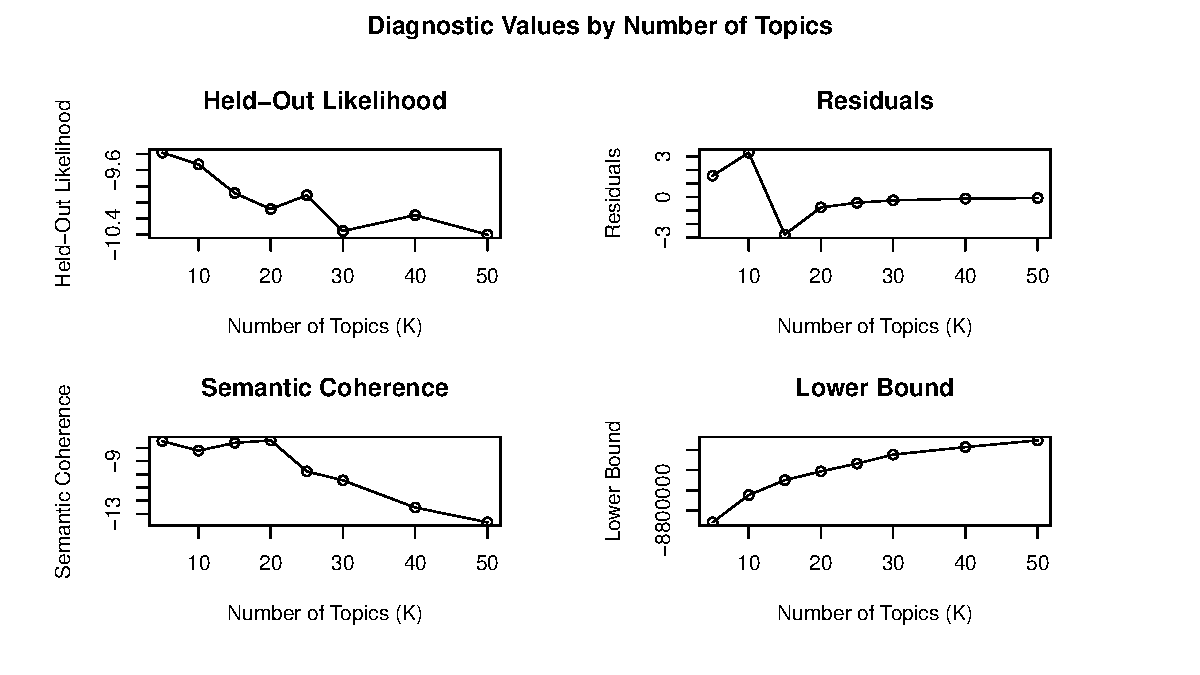
\includegraphics[keepaspectratio]{Maoist_files/figure-pdf/fig-k-search-1.pdf}}

}

\caption{\label{fig-k-search}Result of the quantitative metric K-search}

\end{figure}%

\subsection{Correspondence Analysis}\label{correspondence-analysis}

As a robustness check, I use the Correspondence Analysis (CA) by Nenadic
and Greenacre (\citeproc{ref-c2007}{2007}) as a non-parametric
alternative to compare the trends in Chinese government reports and
party communiques over the past decades. The Correspondence Analysis
performs singular value decomposition on the normalised document-feature
matrix to project the matrix into lower dimensions. In this project, I
reduce the matrix to 2 dimensions for the best visualisation.

There are three reasons for using the Correspondence Analysis rather
than the wordfish by Slapin and Proksch
(\citeproc{ref-slapin2008}{2008}). Firstly, the Correspondence Analysis
allows us to keep more than one dimension, unlike the wordfish.
Secondly, the Correspondence Analysis is much faster to run and can cope
with larger matrices. Thirdly, the first component of Correspondence
Analysis is usually similar to the wordfish results.

\section{Results}\label{results}

\subsection{Structural Topic Model - Topic Prevalence
Effects}\label{structural-topic-model---topic-prevalence-effects}

I ran a structural topic model with \(K=25\) topics on the Chinese
government reports and party communiques with Leader/Premier names and
Government/Party report as prevalence covariates. The reason for not
including any content covariates is that this project focuses on what
topics are mentioned more by each leader/premier rather than which words
they use for each topic. Moreover, adding content covariates
dramatically increases the time of running the model. The topic names
and their Chinese keywords by FREX are presented in
Figure~\ref{fig-stm-plot} in the order of their prevalence in all
documents. The FREX score is higher when the words are both frequent and
exclusive to the topic. It is the harmonic mean of the rank by
probability within topic (frequency) and rank by distribution of topic
given the word (exclusivity). An English version of the keywords with
topic numbers is presented in Figure~\ref{fig-stm-plot-english}.

\begin{figure}[h]

\centering{

\pandocbounded{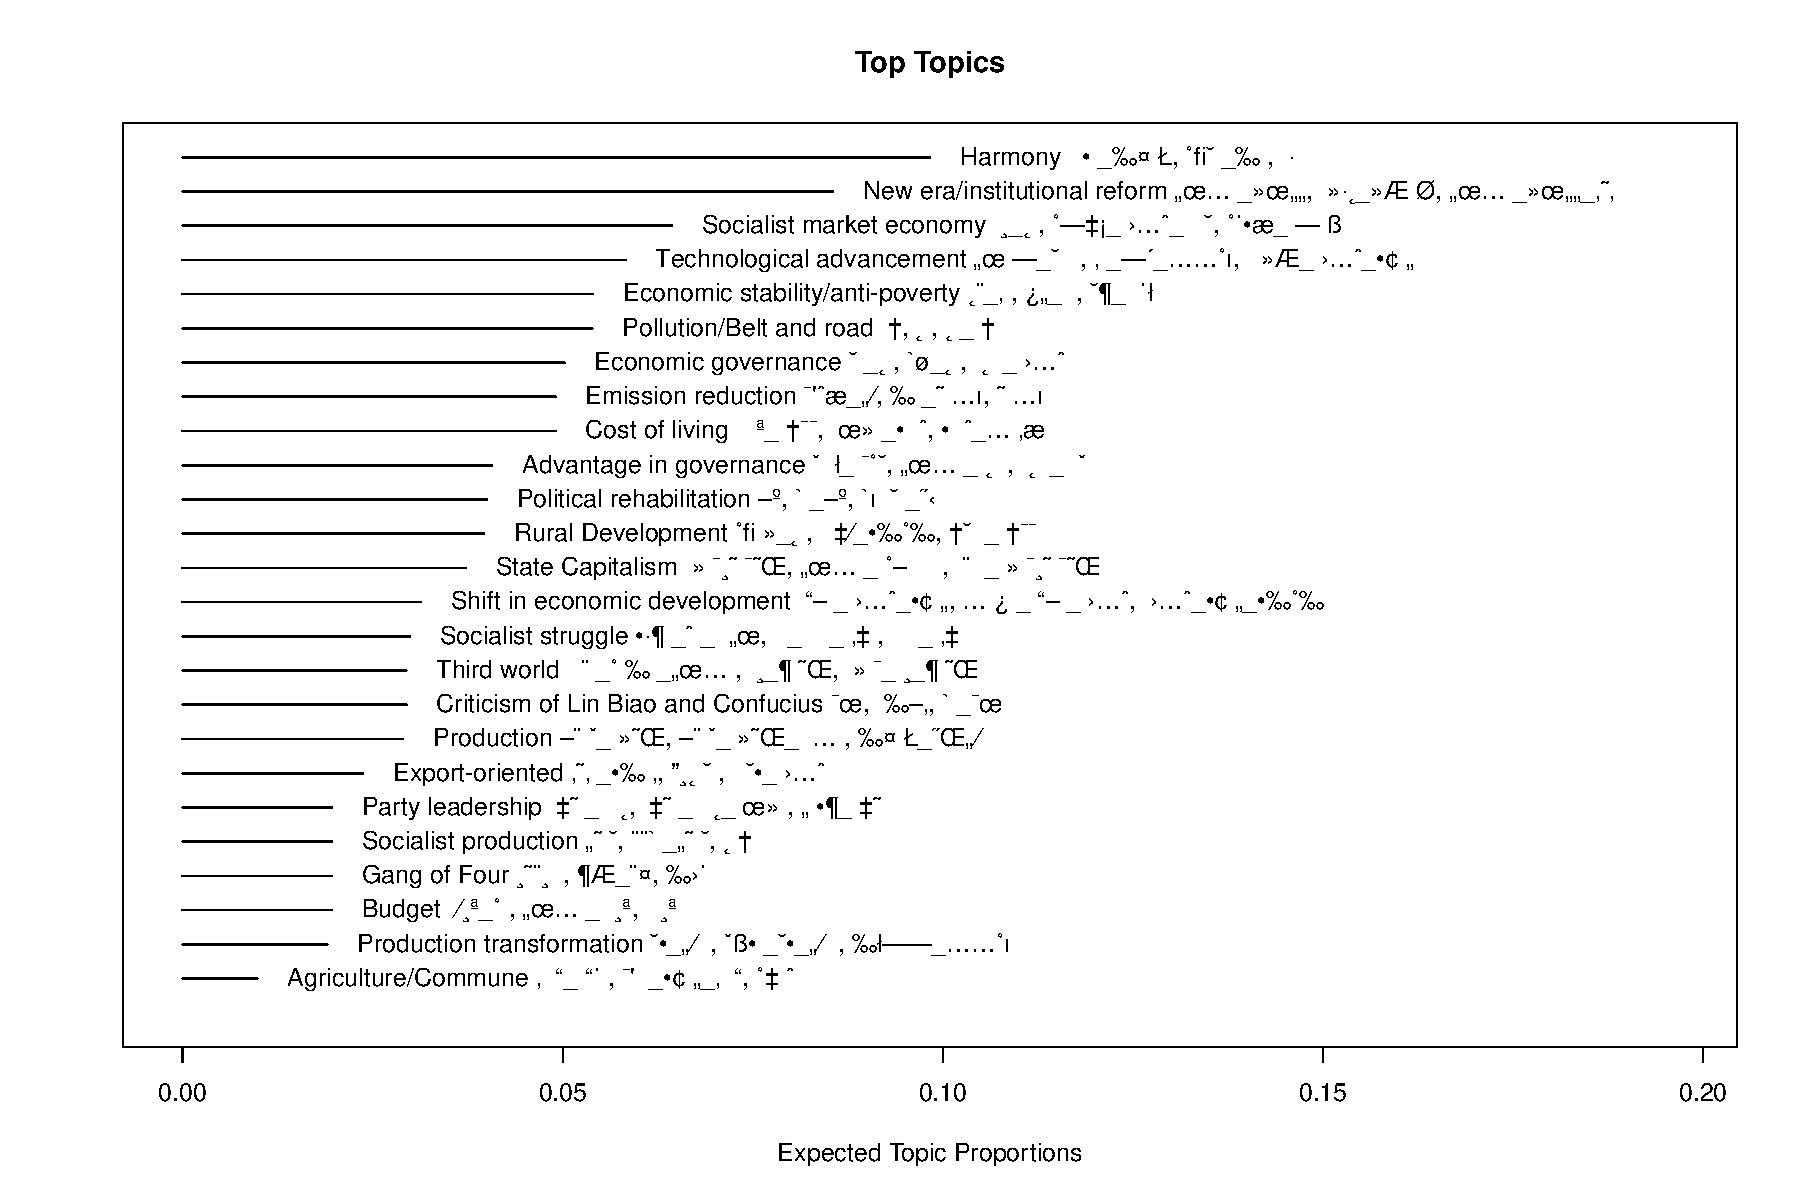
\includegraphics[keepaspectratio]{Maoist_files/figure-pdf/fig-stm-plot-1.pdf}}

}

\caption{\label{fig-stm-plot}Topics in Chinese government reports and
party communiques and related words by FREX}

\end{figure}%

\begin{figure}[h]

\centering{

\pandocbounded{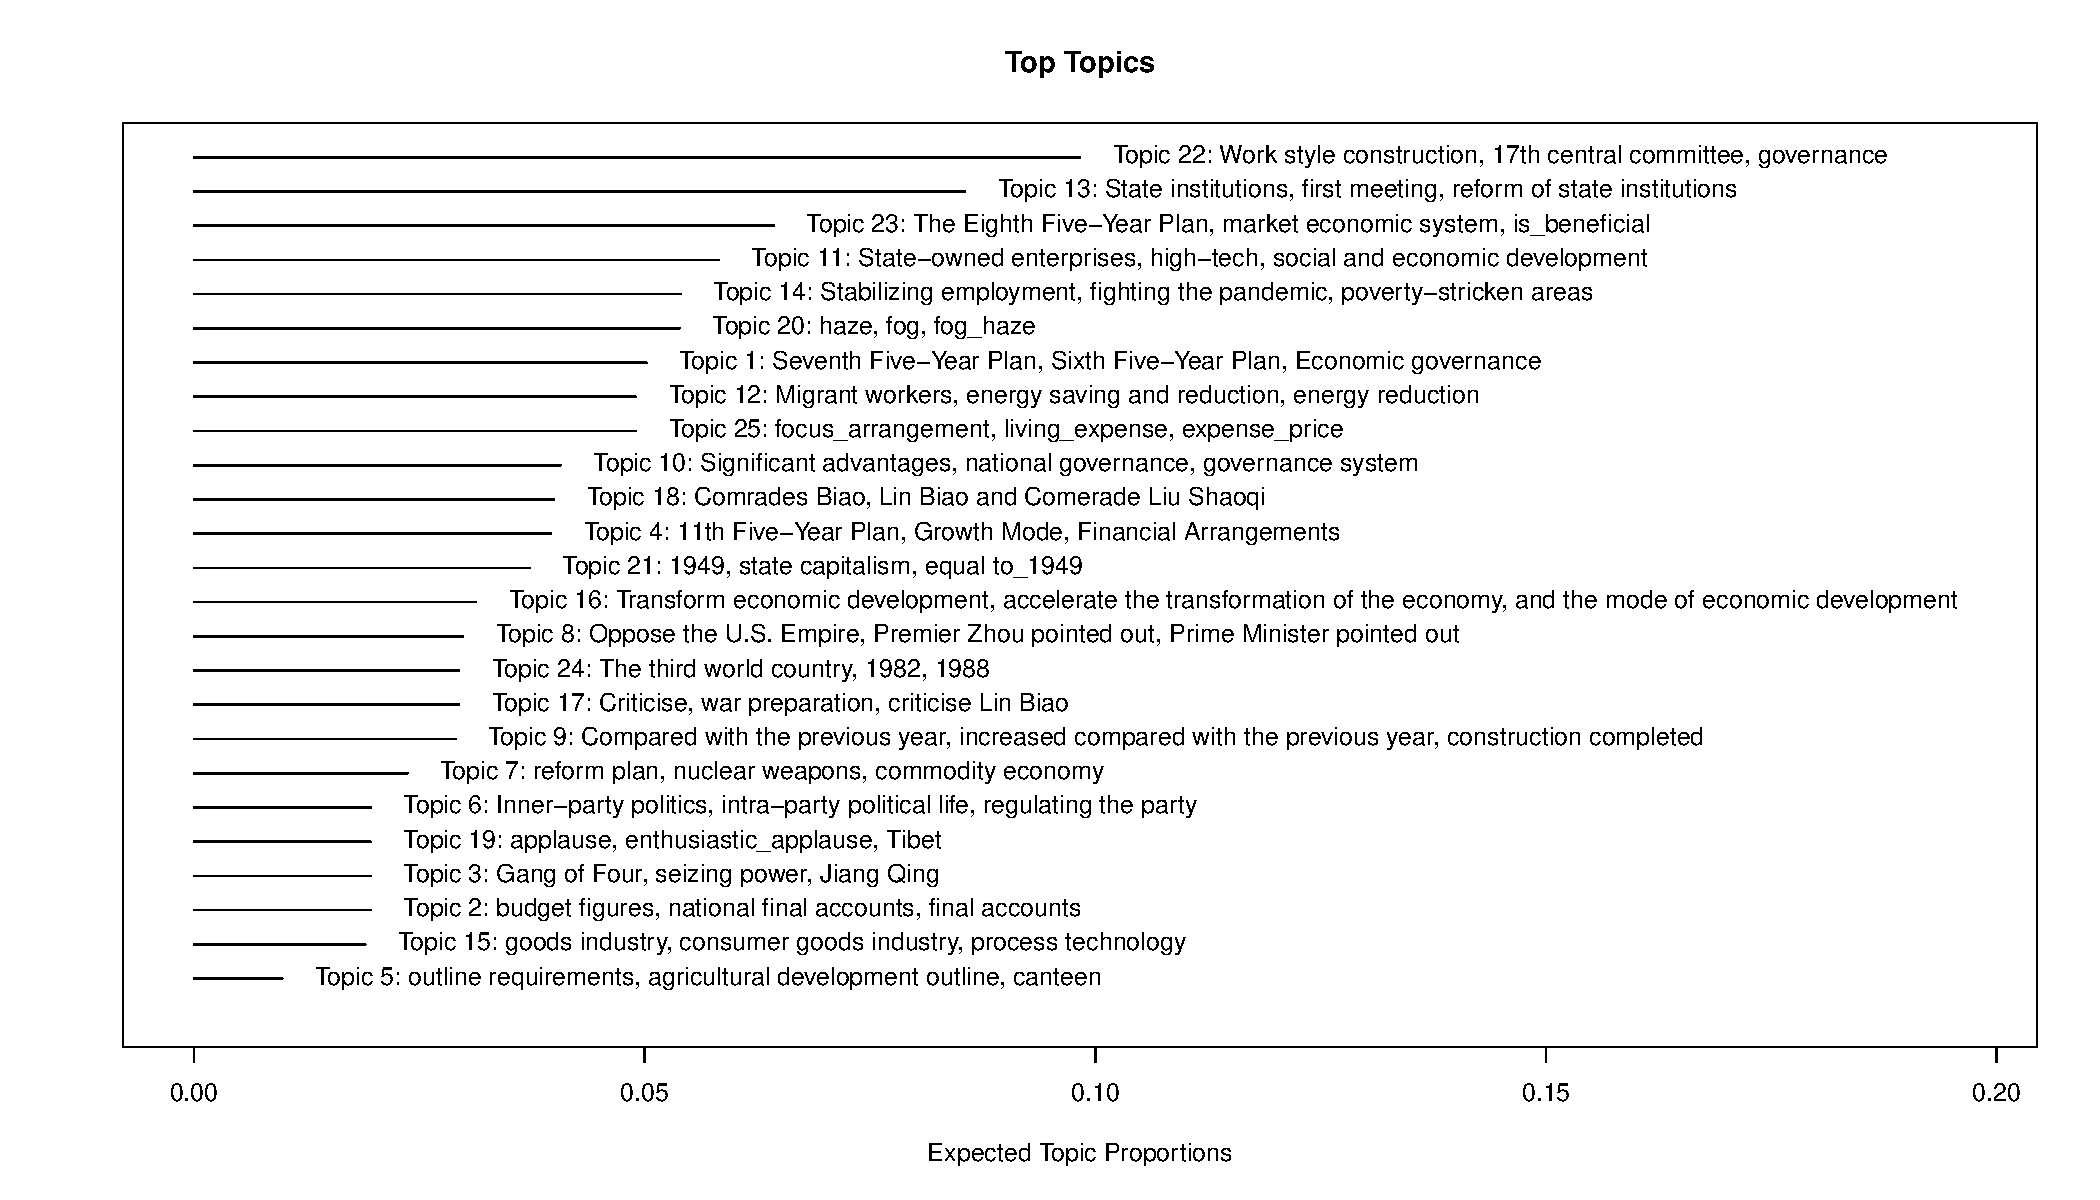
\includegraphics[keepaspectratio]{Maoist_files/figure-pdf/fig-stm-plot-english-1.pdf}}

}

\caption{\label{fig-stm-plot-english}Topics in Chinese government
reports and party communiques and related words by FREX (in English)}

\end{figure}%

The results show that almost all topics correspond to a specific time
period or even a specific leader/premier. However, there tended to be
overlaps between party communiques and government reports when five-year
plans or broad economic planning were of concern. For example, Topic 1,
``Economic governance,'' is closely related to the 6th and 7th Five-Year
Plans, as revealed by the FREX words in
Figure~\ref{fig-stm-plot-english}. The leader associated with these
plans were Deng Xiaoping and the corresponding premiers are Zhao Ziyang
and Lipeng. This is reflected in Figure~\ref{fig-topic1} which shows
higher prevalence effects of them.

\begin{figure}

\centering{

\pandocbounded{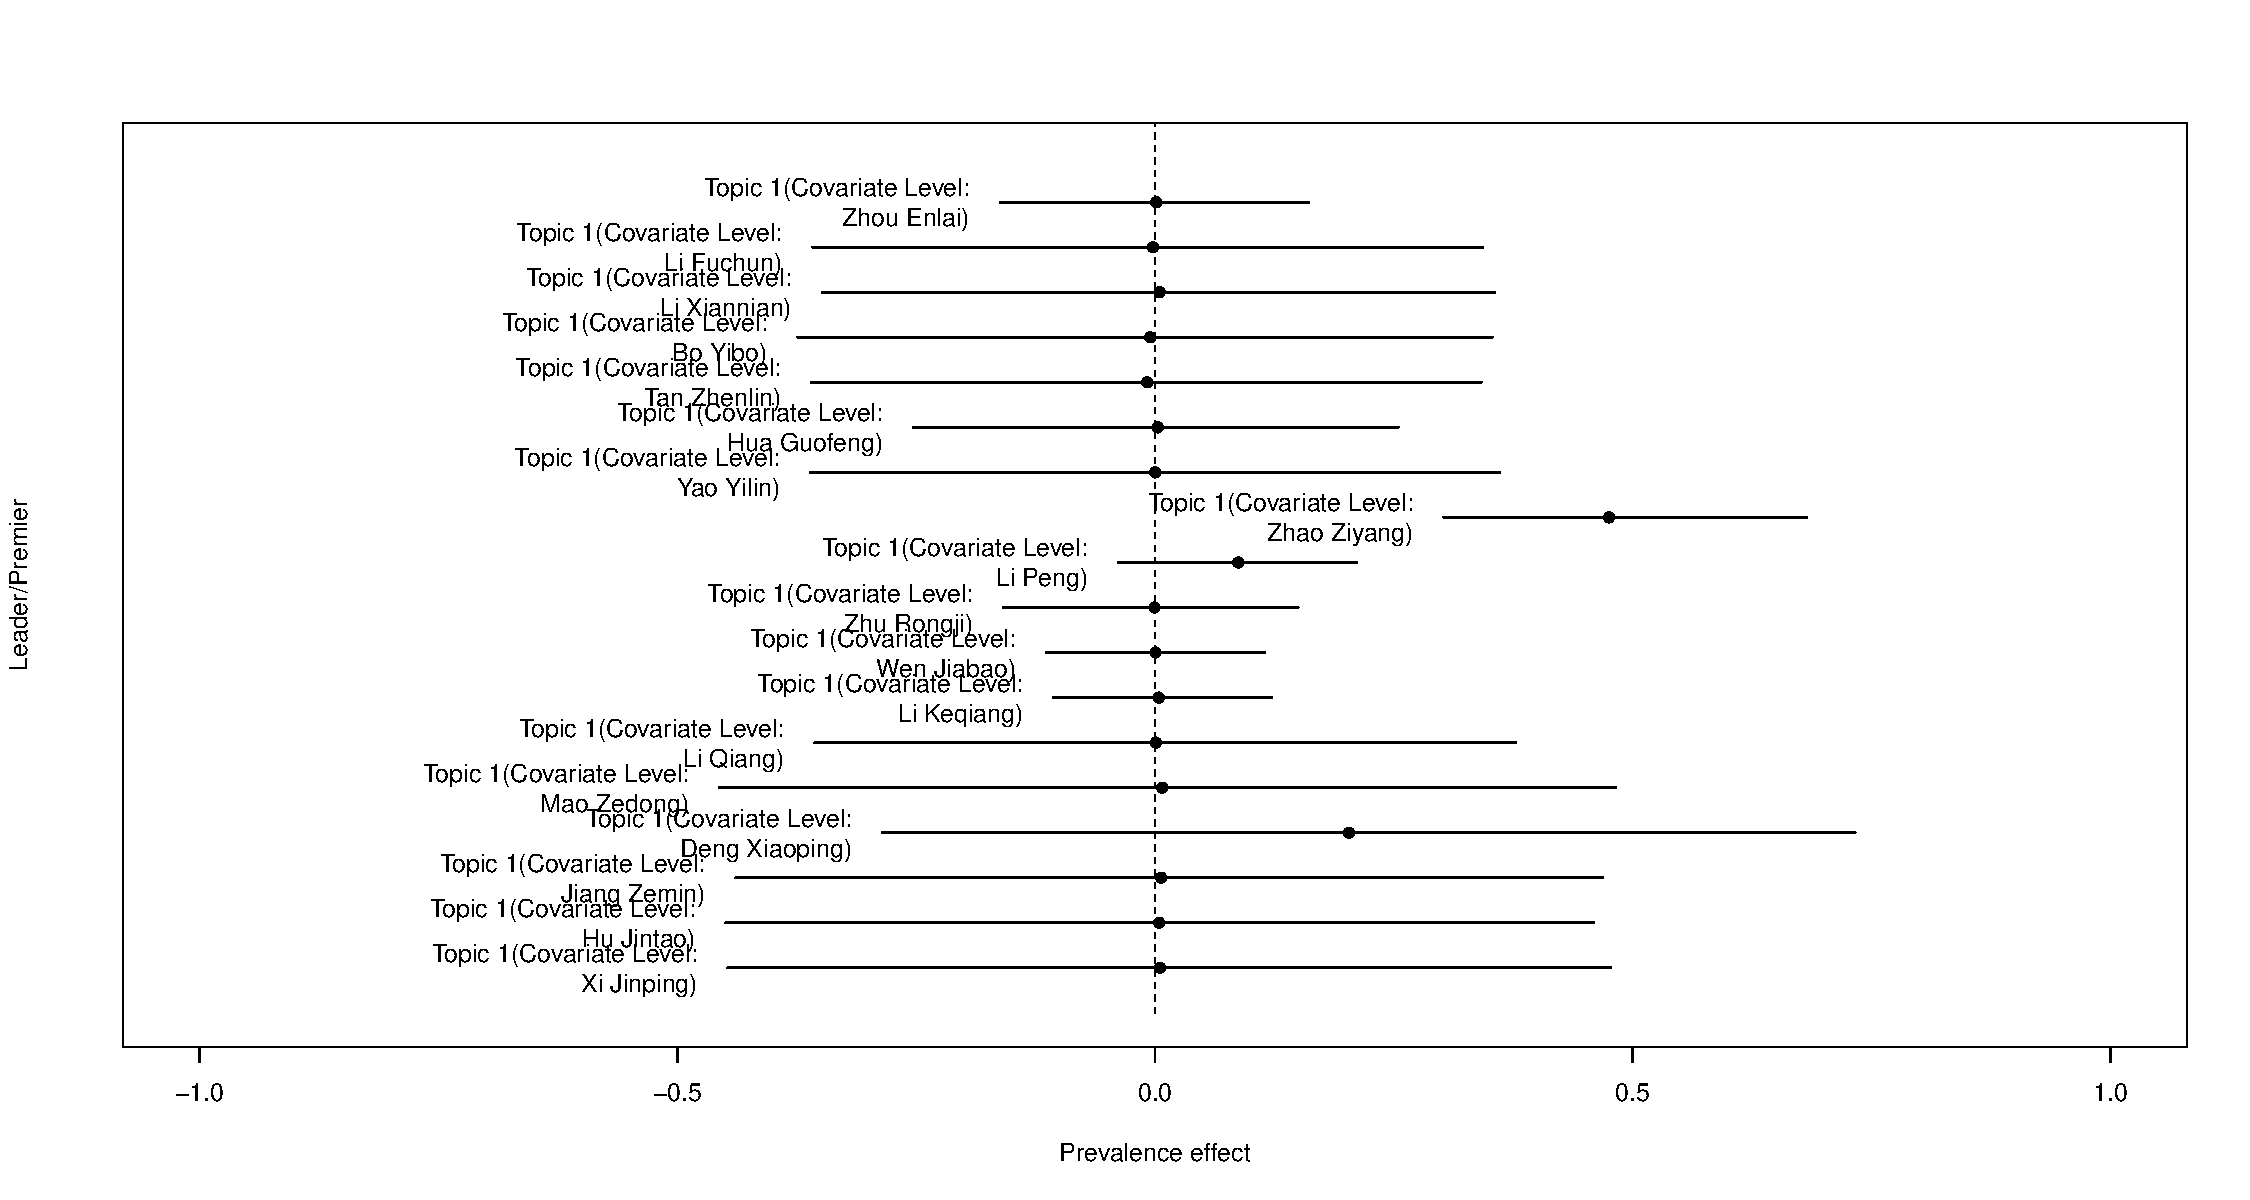
\includegraphics[keepaspectratio]{Maoist_files/figure-pdf/fig-topic1-1.pdf}}

}

\caption{\label{fig-topic1}Topic 1, ``Economic governance,'' in Chinese
government reports and party communiques}

\end{figure}%

Similarly, Topic 4, ``Rural Development,'' is associated with the 11th
Five-Year Plan. The corresponding leader and premier were Hu Jintao and
Wen Jiabao. This is reflected in Figure~\ref{fig-topic4} which shows
higher prevalence effects of them.

\begin{figure}

\centering{

\pandocbounded{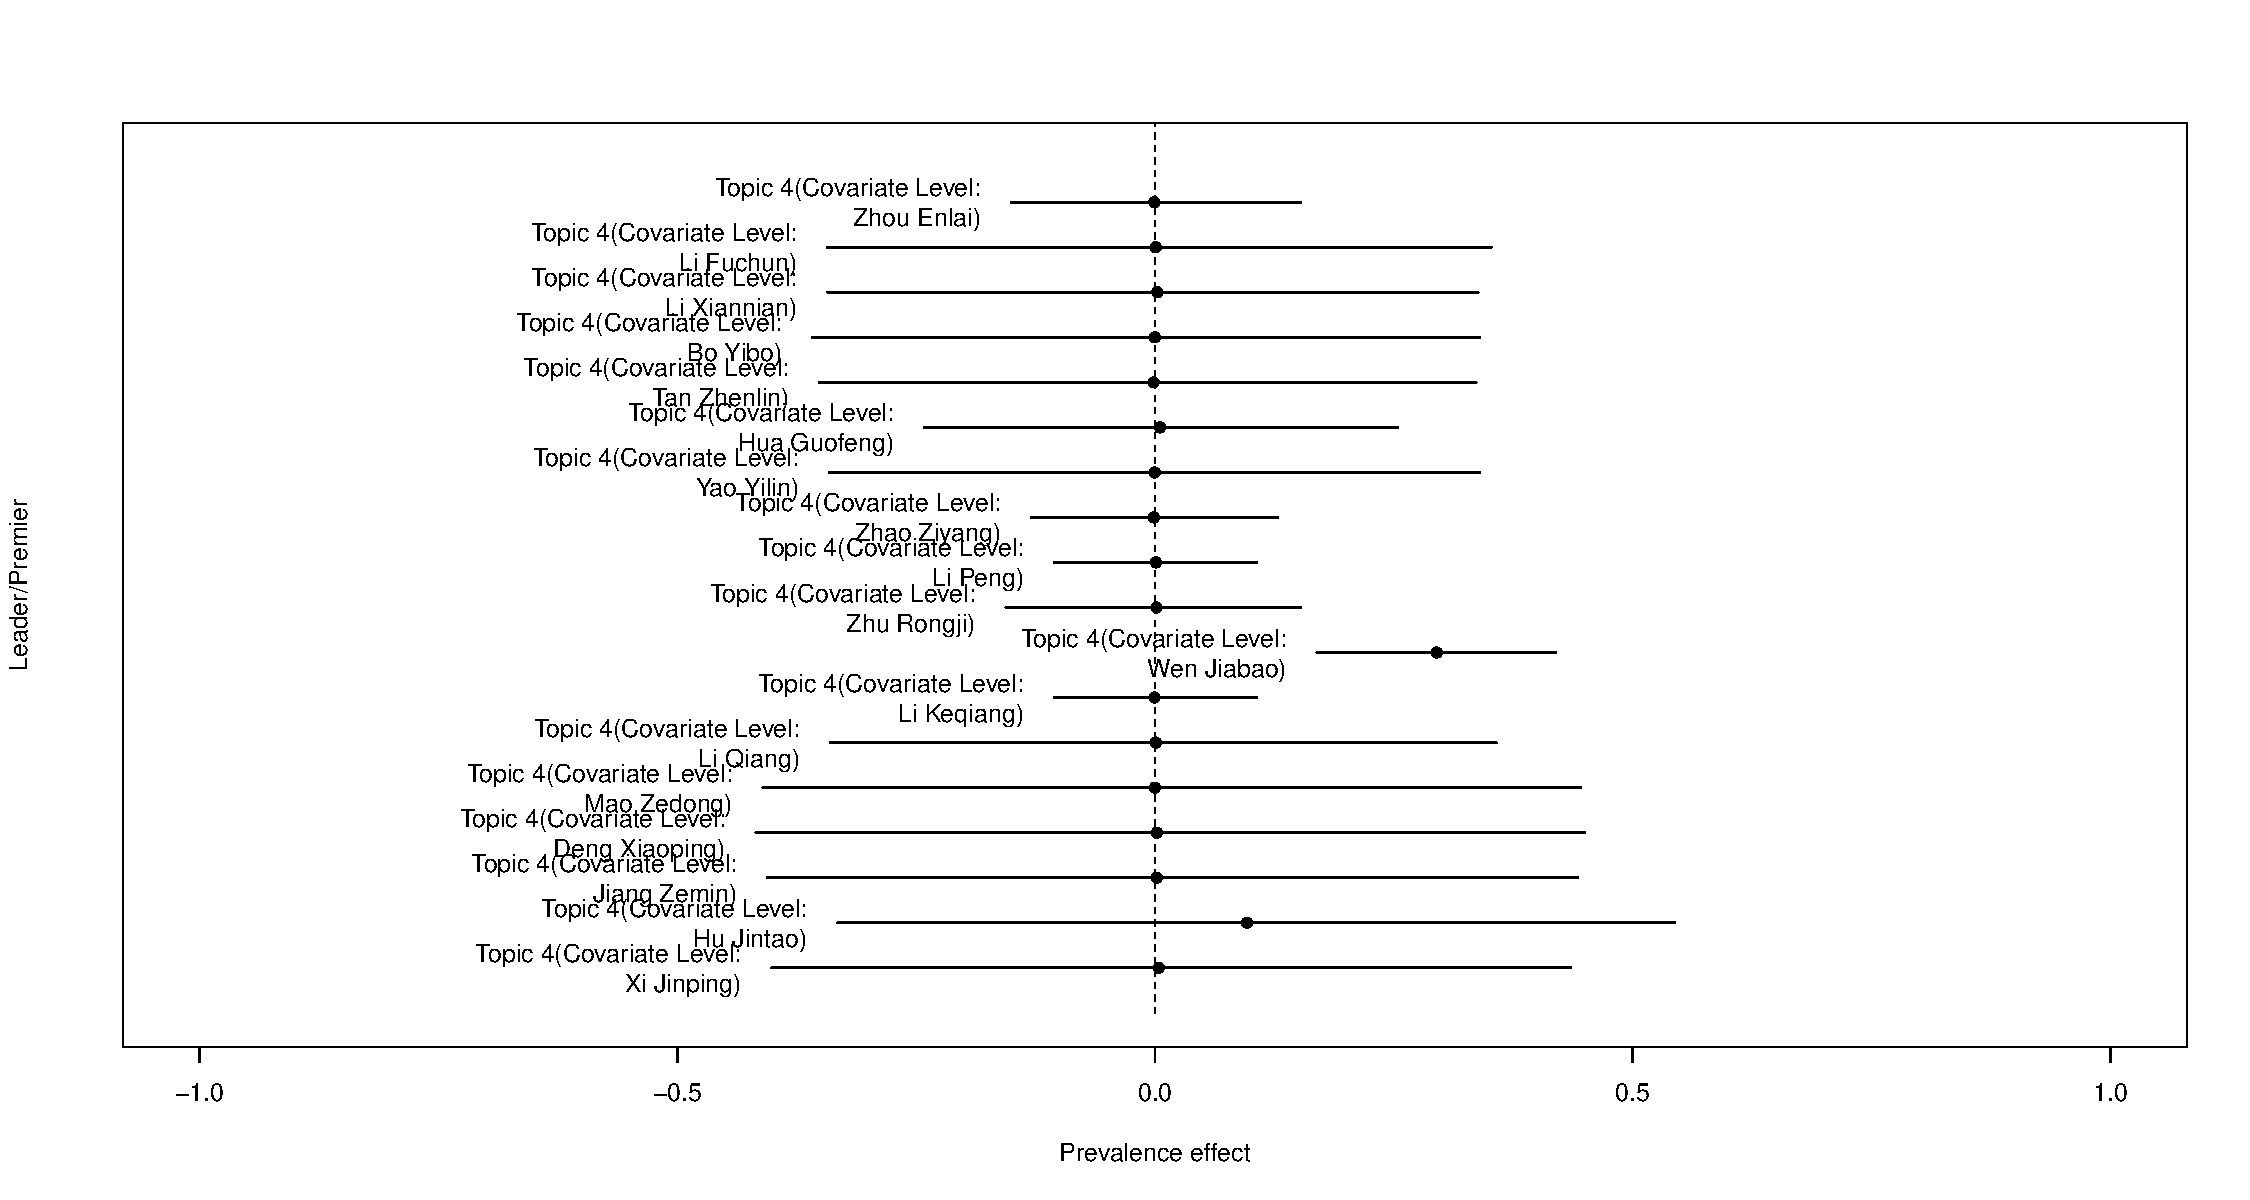
\includegraphics[keepaspectratio]{Maoist_files/figure-pdf/fig-topic4-1.pdf}}

}

\caption{\label{fig-topic4}Topic 4, ``Rural Development,'' in Chinese
government reports and party communiques}

\end{figure}%

However, the interaction between the party and government on economic
planning decreased under Xi Jinping's leadership. Neither the party
communiques nor the government reports emphasised the corresponding
five-year plans. As a result, five-year plans under Xi failed to be
recognised as a distinct topic by the model. The party communiques under
Xi switched to party leadership and intra-party disciplines (Topic 6)
and the government reports focused more on ex tempore economic problems
such as the COVID-19 pandemic and pollution (e.g.~Topic 14 and 20).

As shown in Figure~\ref{fig-topic6}, the leadership of the party and
intra-party discipline has only been emphasized by Xi Jinping. This is
not echoed by his prime ministers, Li Keqiang or Li Qiang.

\begin{figure}

\centering{

\pandocbounded{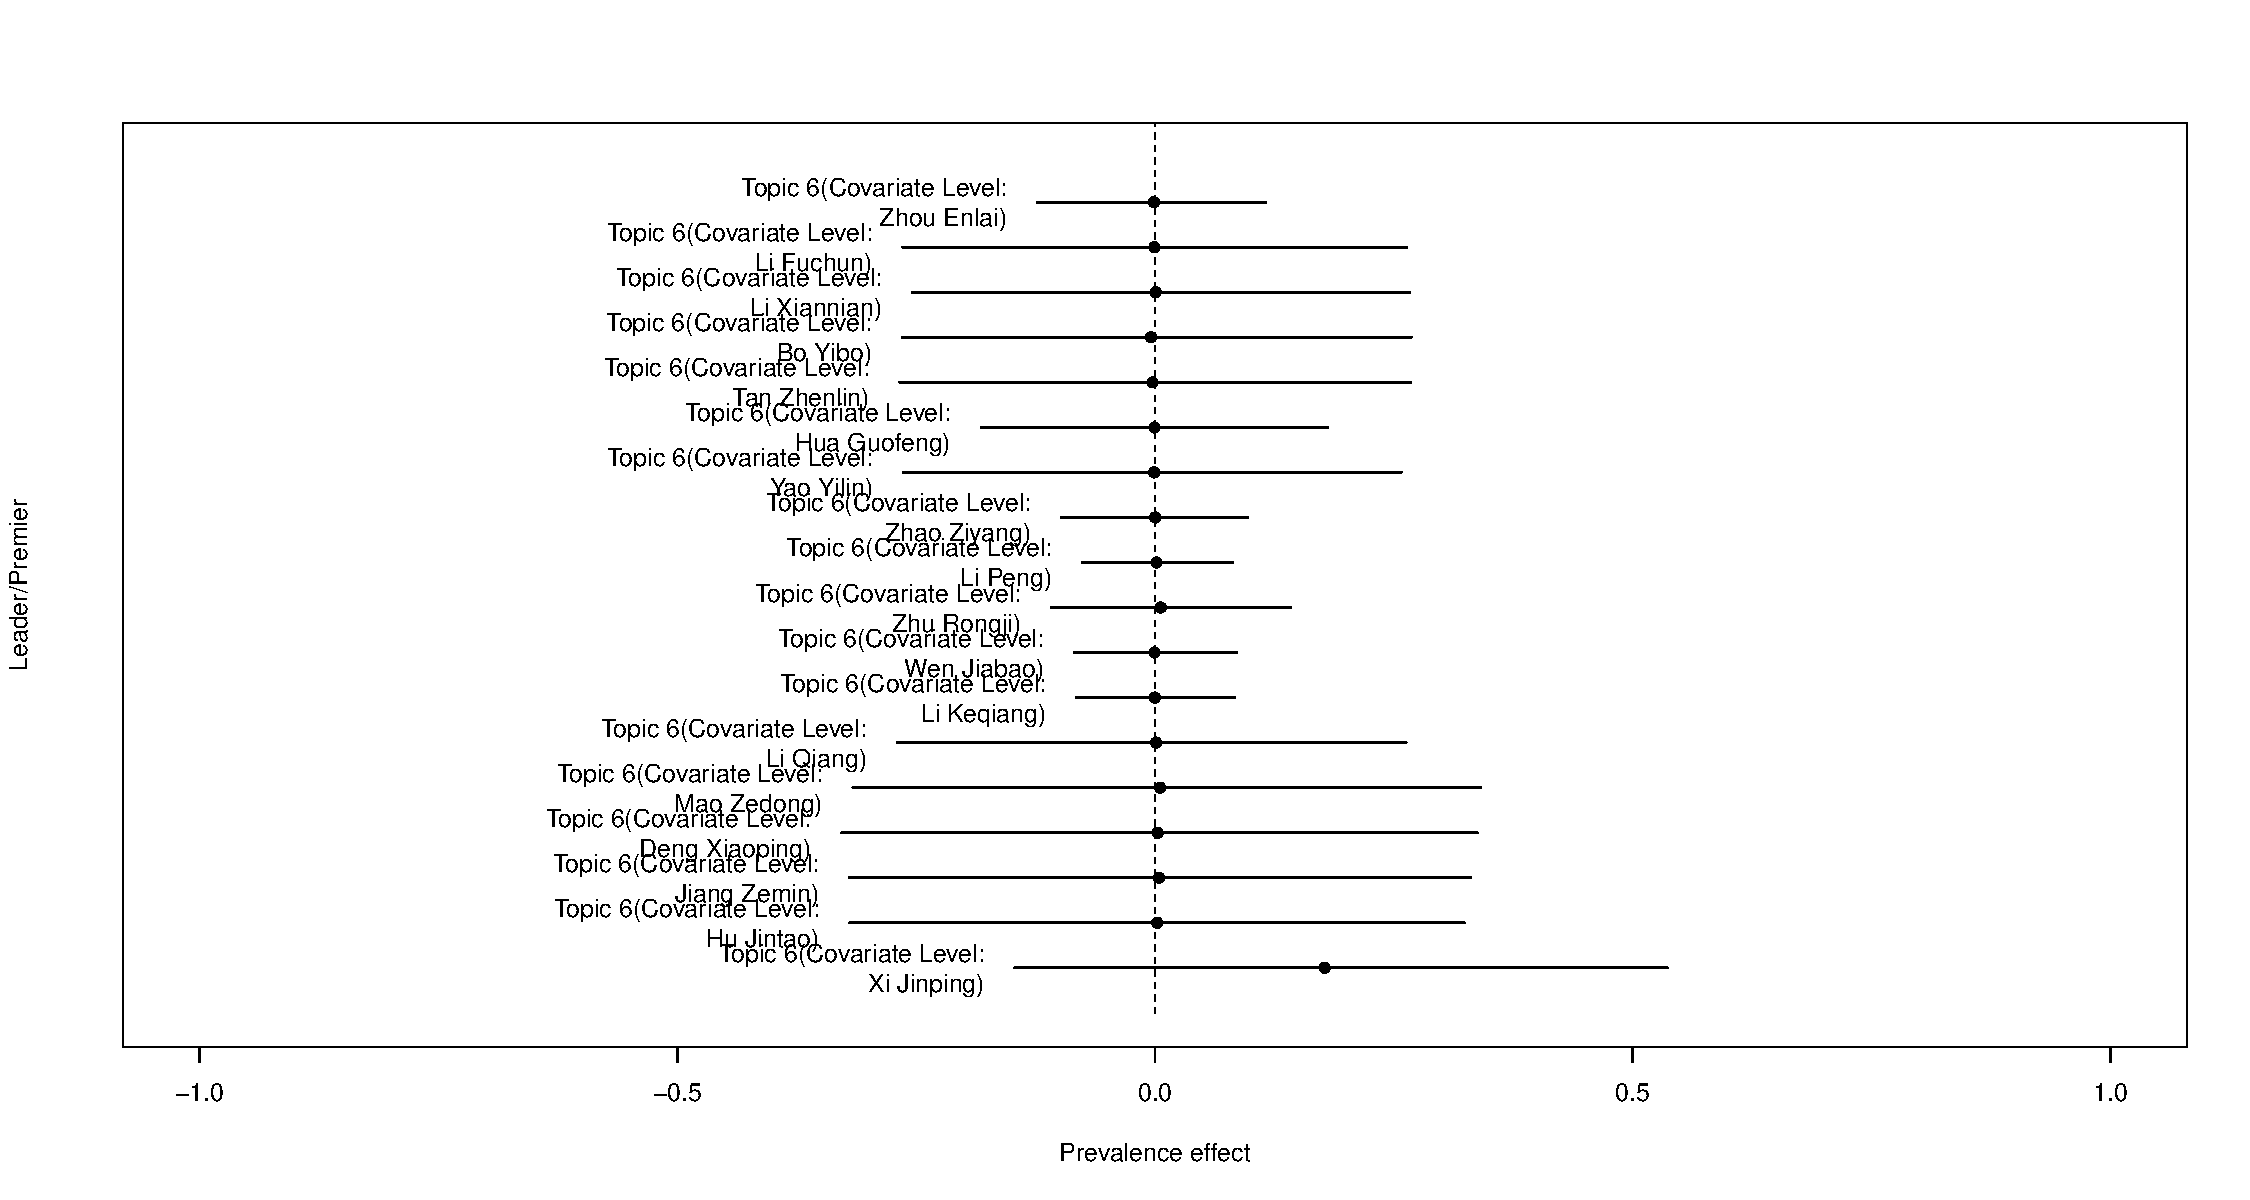
\includegraphics[keepaspectratio]{Maoist_files/figure-pdf/fig-topic6-1.pdf}}

}

\caption{\label{fig-topic6}Topic 6, ``Party leadership,'' in Chinese
government reports and party communiques}

\end{figure}%

On the other hand, Topic 14 (Economic stability/anti-poverty/pandemic)
and Topic 20 (Pollution) are more related to the ex tempore economic
problems that were only mentioned by Premier Li Qiang
(Figure~\ref{fig-topic-14}) and Li Keqiang (Figure~\ref{fig-topic-20}),
respectively. They are not echoed by party communiques under Xi Jinping,
either.

\begin{figure}

\centering{

\pandocbounded{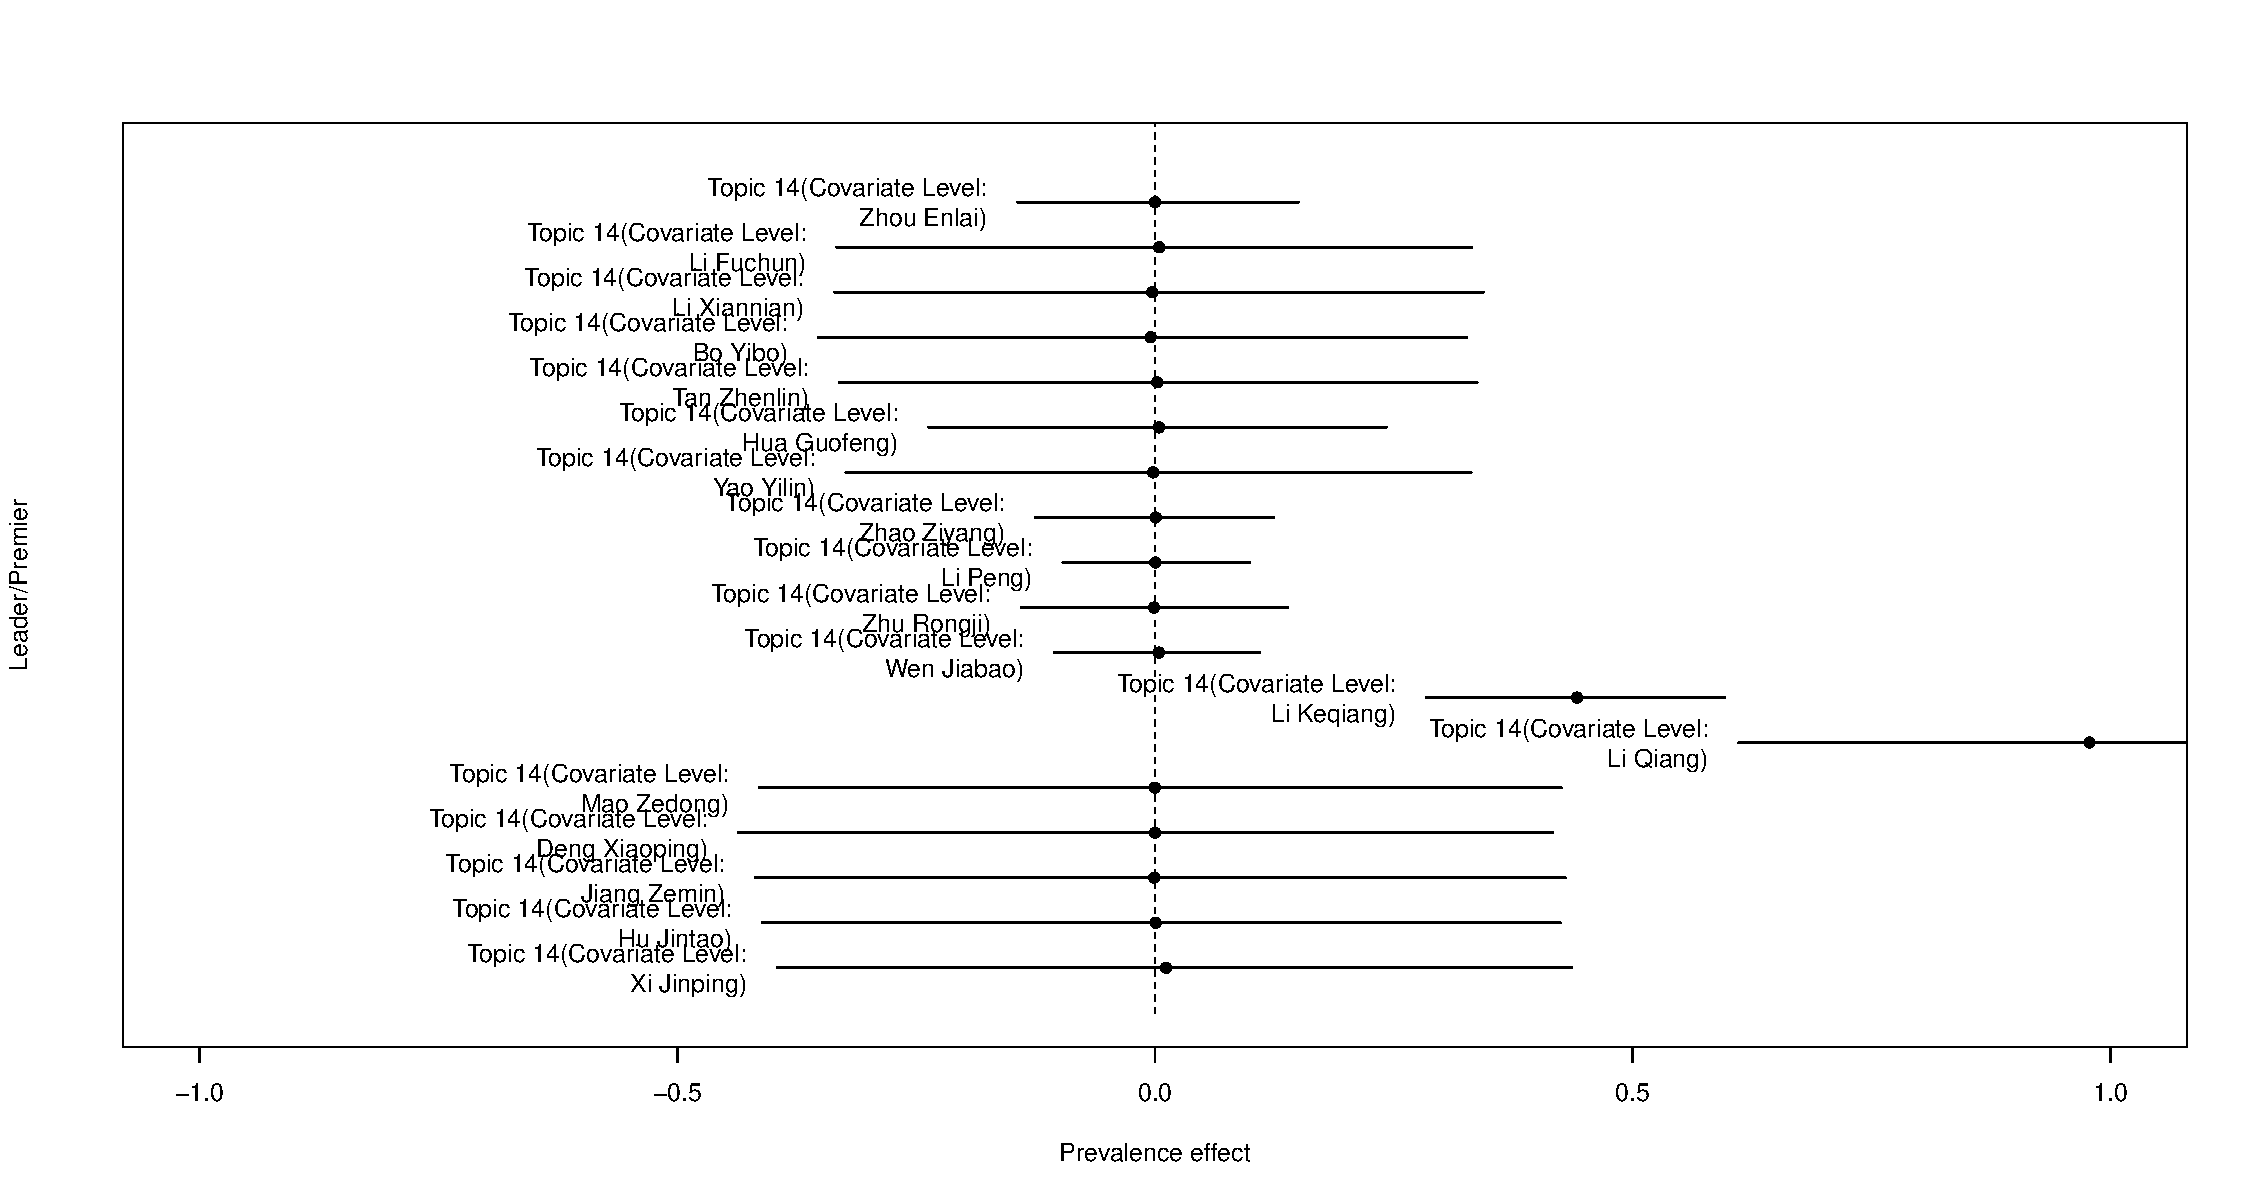
\includegraphics[keepaspectratio]{Maoist_files/figure-pdf/fig-topic-14-1.pdf}}

}

\caption{\label{fig-topic-14}Topic 4, ``Economic
stability/anti-poverty/pandemic,'' in Chinese government reports and
party communiques}

\end{figure}%

\begin{figure}

\centering{

\pandocbounded{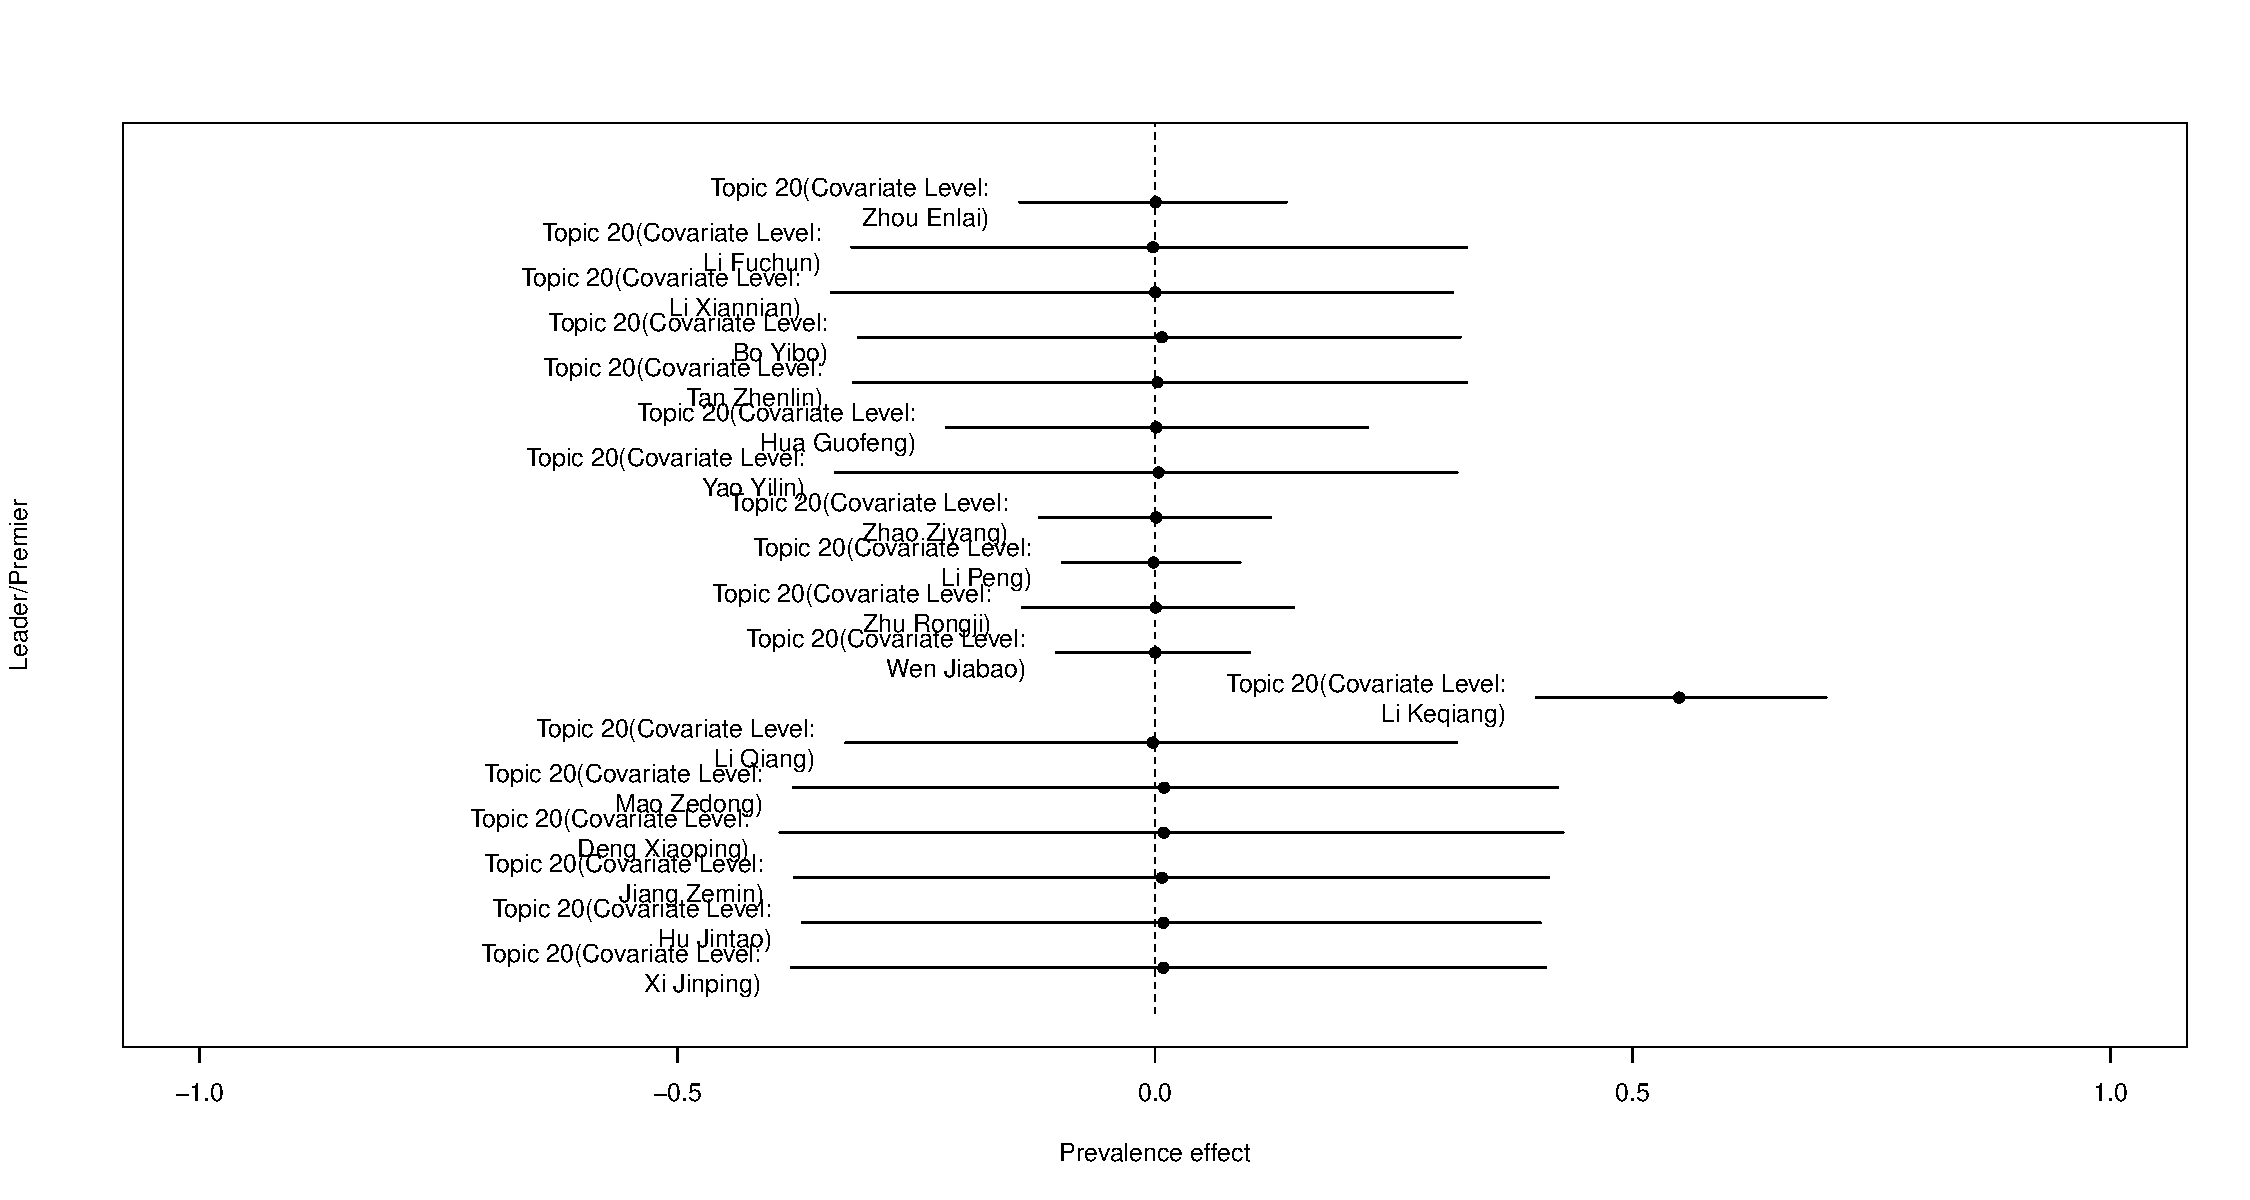
\includegraphics[keepaspectratio]{Maoist_files/figure-pdf/fig-topic-20-1.pdf}}

}

\caption{\label{fig-topic-20}Topic 20, ``Pollution,'' in Chinese
government reports and party communiques}

\end{figure}%

In the topic related to the New Era and institutional reform (Topic 13),
the prevalence has incrementally increased under the past party leaders
since the Reform and Opening-Up, with the prevalence effect of Xi
Jinping being the highest. This is shown in Figure~\ref{fig-topic13}.
This implies that the recent political trends in the party were not
necessarily intiated by Xi Jinping but were rather a continuation of the
previous party leaders.

\begin{figure}

\centering{

\pandocbounded{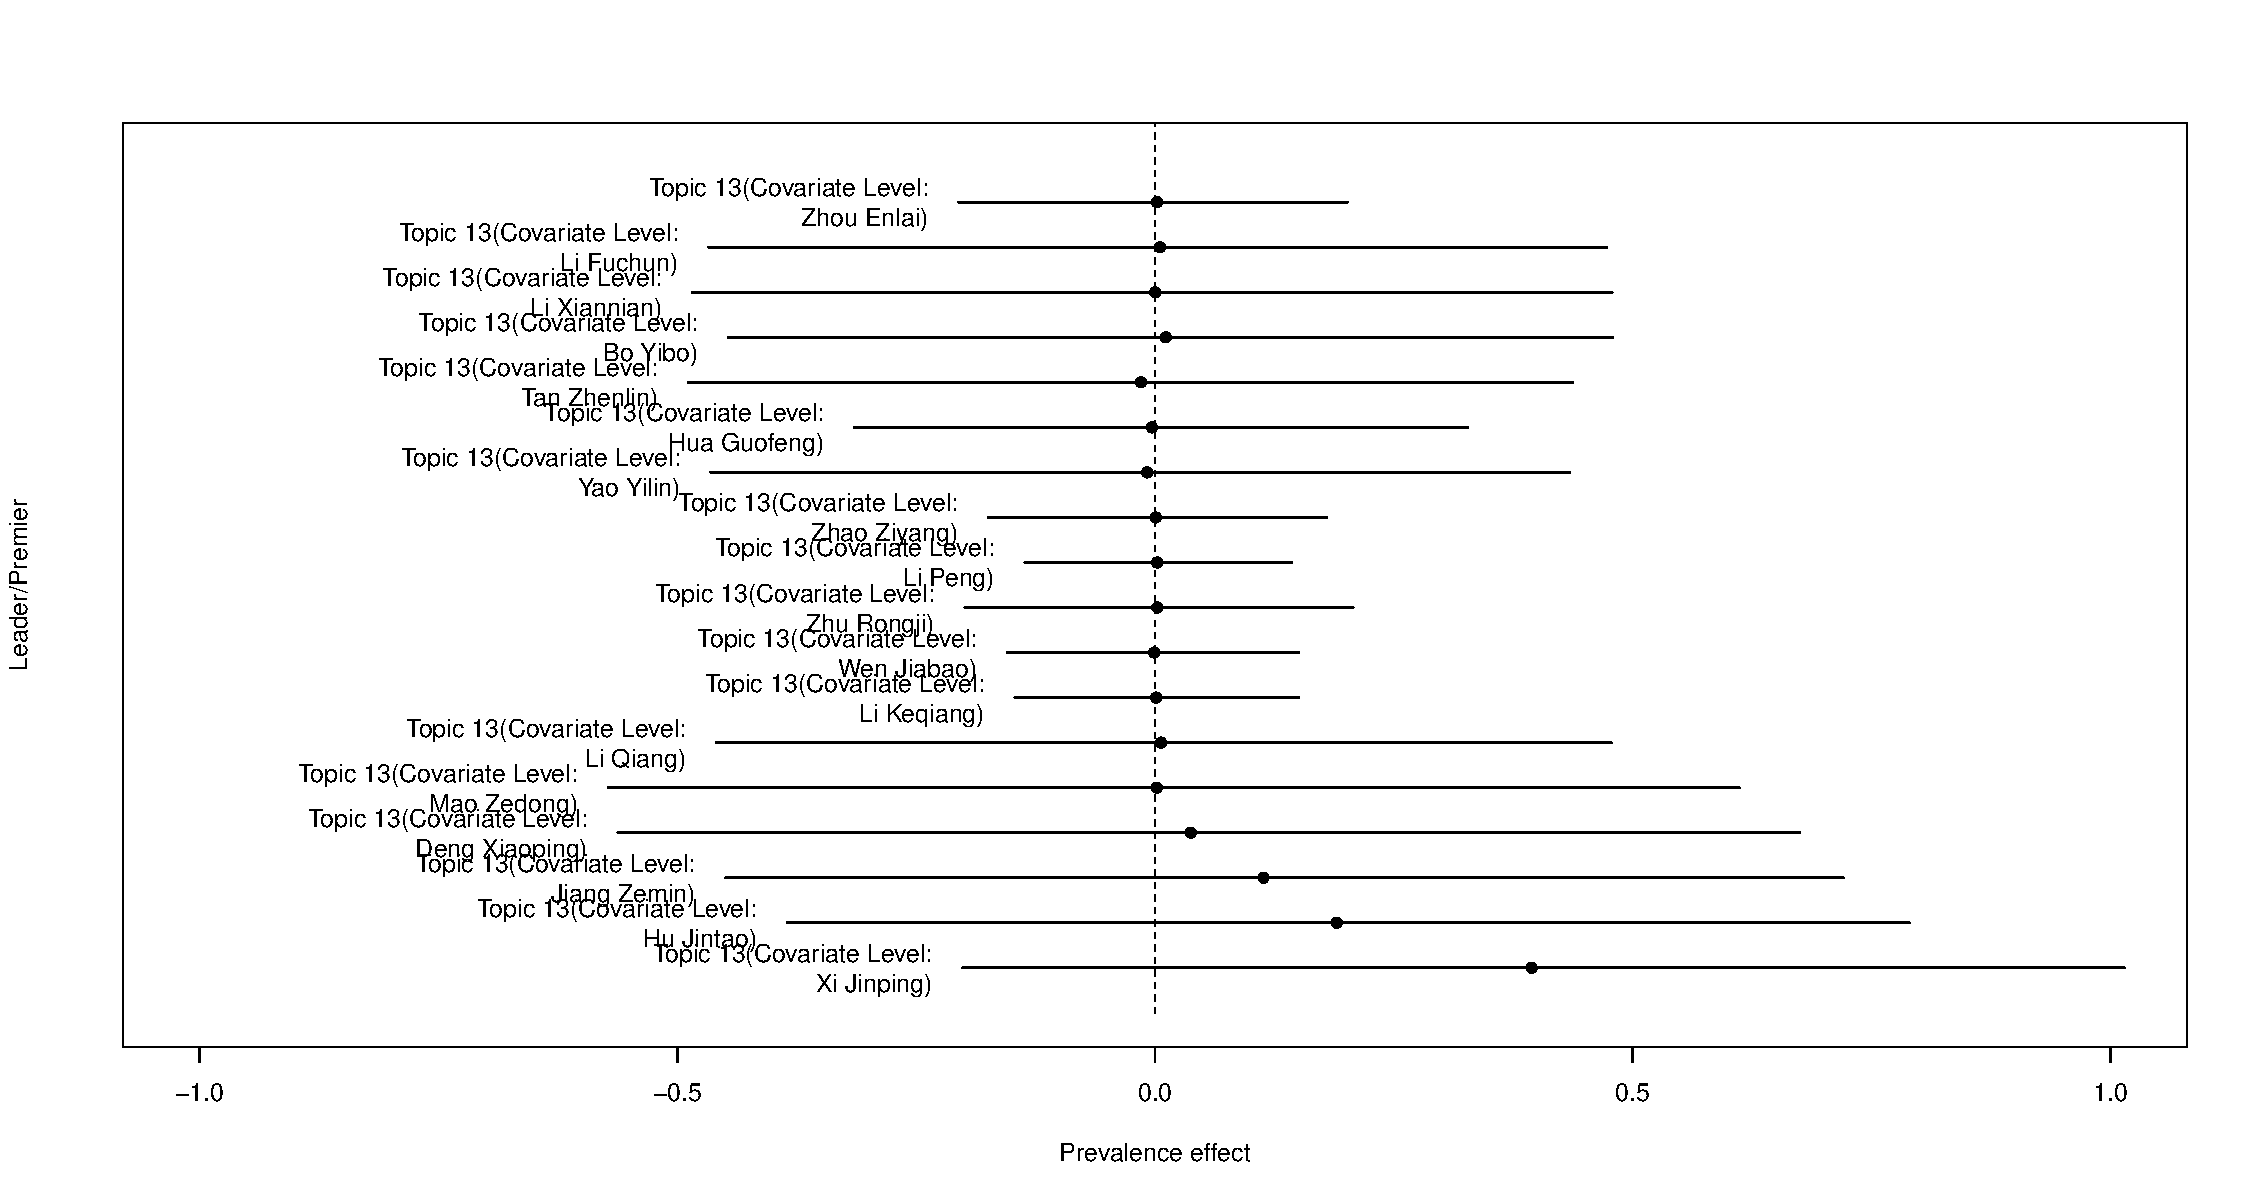
\includegraphics[keepaspectratio]{Maoist_files/figure-pdf/fig-topic13-1.pdf}}

}

\caption{\label{fig-topic13}Topic 13, ``New Era/institutional reform,''
in Chinese government reports and party communiques}

\end{figure}%

In summary, the results of the topic prevalence effects show that the
overlap between party communiques and government reports has decreased
under Xi Jinping's leadership. The party communiques have shifted to
party leadership and intra-party discipline, while the government
reports have focused more on ex tempore economic problems. The recent
political trends in the party were not necessarily initiated by Xi
Jinping but were rather a continuation of the previous party leaders.
These results will be further examined by other methods in the following
sections.

Moreover, there is no evidence that the party communiques or the
government reports under Xi have realigned with the Mao era. There is
almost no overlap between the topics of the Mao era and the Xi era.

\subsection{Structural Topic Model - Topic distribution
agreement}\label{structural-topic-model---topic-distribution-agreement}

One drawback of the prevalence effect analysis is that it only shows
whether or not a topic is more prevalent under a specific
leader/premier. It does not show the extent of similarity of topic
distribution among different leaders/premiers.

The Structural Topic Model conveniently provides the distribution of
topics in each document as a parameter (\(\theta\)). We can use this
information to calculate the similarity of topic distribution among
leaders and their corresponding premiers. The similarity of topic
distribution can be calculated using the Euclidean distance between the
mean topic distribution of each leader and that of their corresponding
premiers. The smaller the distance, the more similar the topic
distribution.

\begin{figure}

\centering{

\pandocbounded{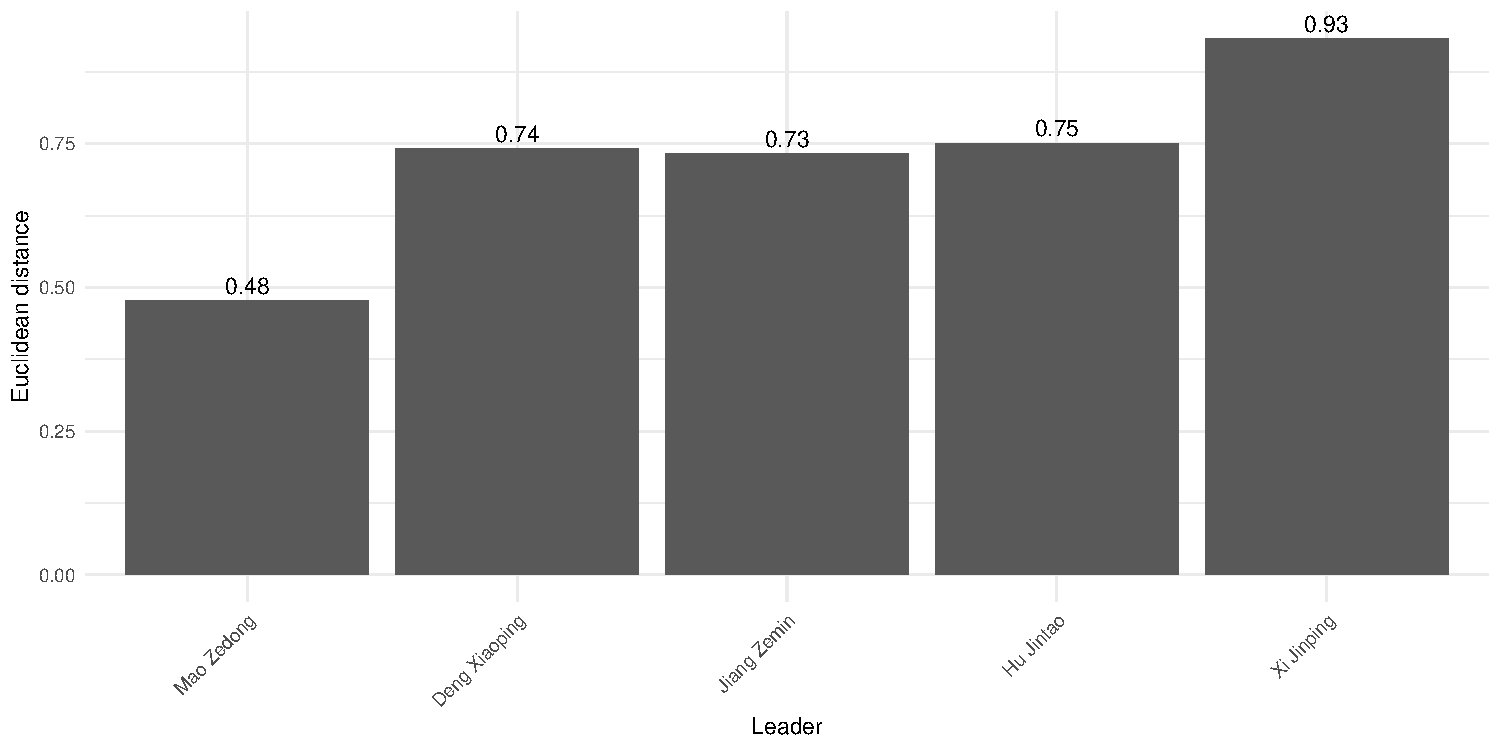
\includegraphics[keepaspectratio]{Maoist_files/figure-pdf/fig-stm-topic-dist-1.pdf}}

}

\caption{\label{fig-stm-topic-dist}Euclidean distance of mean topic
distribution among leaders and their corresponding premiers}

\end{figure}%

Figure~\ref{fig-stm-topic-dist} shows the similarity of topic
distribution among leaders and their corresponding premiers. The results
show that the topic distribution of Xi Jinping and his premiers is the
most dissimilar, followed by Hu Jintao and Wen Jiabao. The topic
distribution of Mao Zedong and his premiers is the most similar. This
confirms our previous results that the overlap between party communiques
and government reports has decreased under Xi Jinping's leadership.

\subsection{Correspondence analysis}\label{correspondence-analysis-1}

The first dimension of the Correspondence Analysis scores by year and
party/government is plotted in Figure~\ref{fig-ca}. The Correspondence
Analysis results confirm that the party communiques and government
reports were largely overlapped under Mao, Deng and Jiang, but diverged
under Xi.

However, the Correspondence Analysis results disagree with the STM
results in that the former imply that the divergence started in the late
Jiang or Hu era, whereas the latter suggest that the divergence has only
been visible under Xi.

More interestingly, the first dimension of the Correspondence Analysis
seems to capture the shift in the left-right political spectrum. A lower
score on the first dimension indicates a more left-leaning political
stance, while a higher score indicates a more right-leaning stance.
Specifically, Reform and Opening-Up since 1978 marked a shift to the
right in both party communiques and government reports. While the
government communiques continued to shift to the right by emphasising
economic development and entrepreneurship, the party communiques
\emph{ceased to} shift to the right by focusing on party leadership and
intra-party discipline under Xi. This divergence in trends is
unprecedented in the history of the PRC and is a promising area for
further research.

However, the second component is not shown here as I have not found a
meaningful interpretation for it. Nevertheless, the results for the
second component are provided in Appendix~\ref{sec-second-ca}.

\begin{figure}

\centering{

\pandocbounded{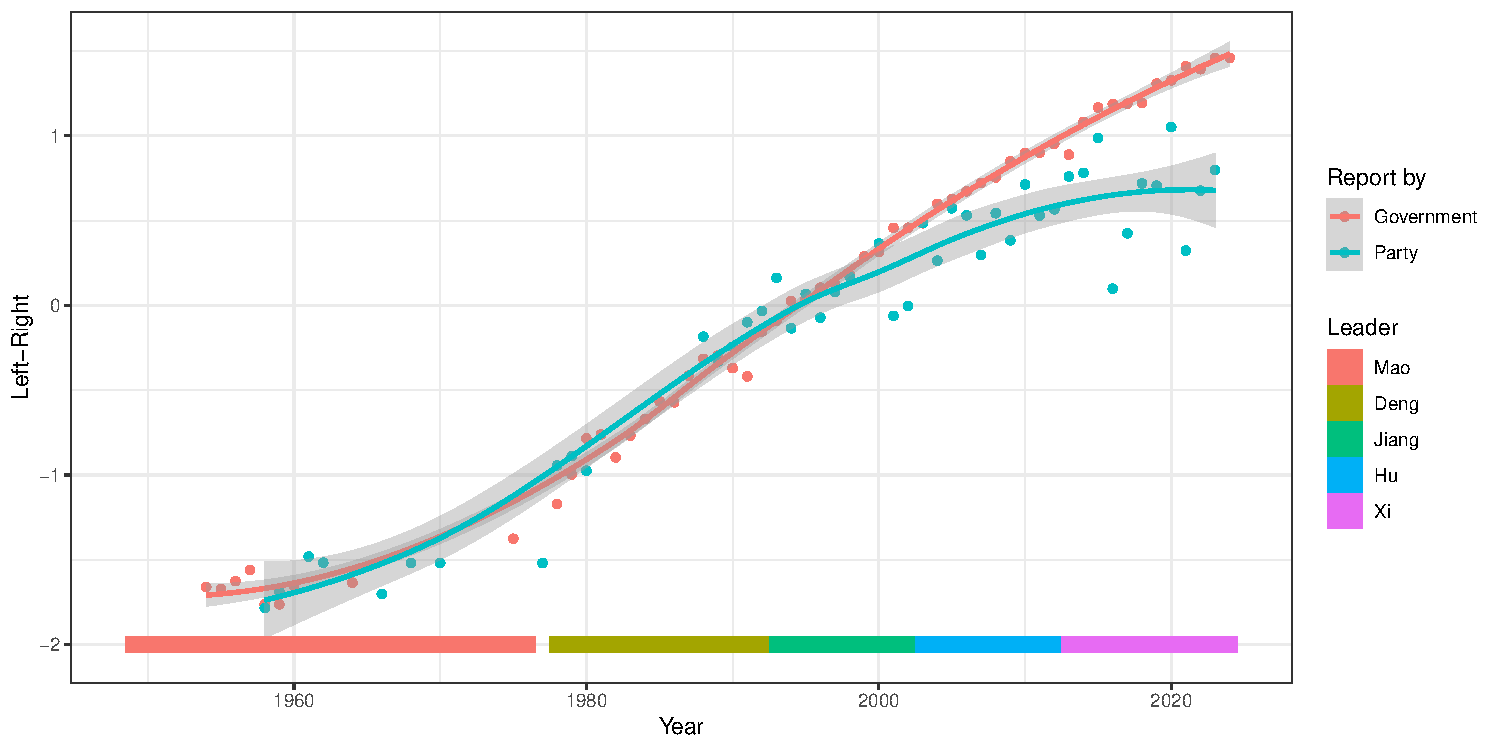
\includegraphics[keepaspectratio]{Maoist_files/figure-pdf/fig-ca-1.pdf}}

}

\caption{\label{fig-ca}Correspondence analysis of Chinese government
reports and party communiques (first dimension)}

\end{figure}%

\section{Conclusions}\label{conclusions}

In conclusion, there is no evidence of a realignment with the Mao era in
the party communiques or government reports under Xi Jinping. On the
contrary, the style of the party communiques and government reports is
more of a continuation of the Hu era. Therefore, the hypothesis that Xi
Jinping is moving toward a more Maoist style and putting an end to the
Reform and Opening-Up era is not supported by our data of party
communiques and government reports. It is true that the topics in party
communiques and government reports under Xi differ from those under his
predecessors, but the topics in these reports differed among his
predecessors after all. In terms of the left-right political spectrum,
the party communiques merely \emph{ceased} to shift to the right, rather
than shifted to the left, under Xi Jinping. More interestingly, the
government reports continued to shift to the right.

The divergence in the topic distribution of party communiques and
government reports under Xi Jinping is unprecedented in the history of
the PRC, and very counter-intuitive. This is a promising area for
further research. The party communiques ceased to shift to the right by
focusing on party leadership and intra-party discipline under Xi, while
the government reports continued to shift to the right by emphasising
economic development and entrepreneurship. This is counter-intuitive to
the wide-spread belief that the party is increasingly intervening in the
economy while the State Council is losing its autonomy. Nevertheless,
the divergence should not be over-interpreted, as the institutional and
personnel changes are much more substantial than public reports when
assessing the party-government power dynamics in China.

One source of divergence is the downplaying of the five-year plans,
which had been a key area of overlap between party communiques and
government reports under Mao, Deng and Jiang. This fall in economic
planning is echoed by the fact that the government reports under Xi have
been increasingly focused on ex tempore economic problems such as
environmental pollution and COVID-19, which are more practical rather
than strategic issues. This is in line with the speculation that the
State Council is subdued and marginalised by the party under Xi.

\section*{References}\label{references}
\addcontentsline{toc}{section}{References}

\phantomsection\label{refs}
\begin{CSLReferences}{1}{0}
\bibitem[\citeproctext]{ref-blei2007}
Blei, David M., and John D. Lafferty. 2007. {``A Correlated Topic Model
of Science.''} \emph{The Annals of Applied Statistics} 1 (1).
\url{https://doi.org/10.1214/07-aoas114}.

\bibitem[\citeproctext]{ref-blei2003}
Blei, David M., Andrew Y. Ng, and Michael I. Jordan. 2003. {``Latent
Dirichlet Allocation.''} \emph{Journal of Machine Learning Research} 3
(Jan): 993--1022.

\bibitem[\citeproctext]{ref-chen2023}
Chen, Yuchen, Alex Jiahong Lu, and Angela Xiao Wu. 2023. {``{`}China{'}
as a {`}Black Box?{'} Rethinking Methods Through a Sociotechnical
Perspective.''} \emph{Information, Communication \& Society} 26 (2):
253--69. \url{https://doi.org/10.1080/1369118x.2022.2159488}.

\bibitem[\citeproctext]{ref-CPPCC2023}
CPPCC. 2023.
{``习近平在广东考察时强调:坚定不移全面深化改革扩大高水平对外开放
在推进中国式现代化建设中走在前列 {[}During His Inspection in Guangdong,
Xi Jinping Emphasized: Unswervingly Comprehensively Deepen Reform and
Expand High-Level Opening up to the Outside World, and Be at the
Forefront of Promoting Chinese-Style Modernization.{]}.''}
\url{https://www.gov.cn/yaowen/2023-04/13/content_5751308.htm}.

\bibitem[\citeproctext]{ref-Horsley2023}
Horsley, Jamie. 2023. {``What {Is} the {State} of the {Chinese}
{State}?''}
\url{https://thediplomat.com/2023/09/what-is-the-state-of-the-chinese-state/}.

\bibitem[\citeproctext]{ref-Hsu2023}
Hsu, Sara. 2023. {``Is {China}'s {Reform} and {Opening} {Era} {Over}?''}
\url{https://thediplomat.com/2023/02/is-chinas-reform-and-opening-era-over/}.

\bibitem[\citeproctext]{ref-jiang2021}
Jiang, Yan. 2021. {``Diachronic Lexical Features of Chinese Government
Work Reports: A Text Mining Approach.''} \emph{Advances in Social
Science, Education and Humanities Research}.
\url{https://doi.org/10.2991/assehr.k.210407.140}.

\bibitem[\citeproctext]{ref-Matson2022}
Matson, Emily. 2022. {``Why It's Misleading to Call {Xi} {Jinping} the
{`New {Mao}'}.''}
\url{https://nuvoices.com/2022/10/03/why-its-misleading-to-call-xi-jinping-the-new-mao/}.

\bibitem[\citeproctext]{ref-Milanovic2023}
Milanovic, Branko. 2023. {``Xi {Jinping} Is Not {Mao} Reborn.''}
\emph{UnHerd}.
\url{https://unherd.com/2023/12/xi-jinping-is-not-mao-reborn/}.

\bibitem[\citeproctext]{ref-c2007}
Nenadic, Oleg, and Michael Greenacre. 2007. {``Correspondence Analysis
in{\emph{R}}, with Two- and Three-Dimensional Graphics:
The{\textbf{ca}}Package.''} \emph{Journal of Statistical Software} 20
(3). \url{https://doi.org/10.18637/jss.v020.i03}.

\bibitem[\citeproctext]{ref-roberts2014}
Roberts, Margaret E., Brandon M. Stewart, Dustin Tingley, Christopher
Lucas, Jetson Leder-Luis, Shana Kushner Gadarian, Bethany Albertson, and
David G. Rand. 2014. {``Structural Topic Models for Open{-}Ended Survey
Responses.''} \emph{American Journal of Political Science} 58 (4):
1064--82. \url{https://doi.org/10.1111/ajps.12103}.

\bibitem[\citeproctext]{ref-slapin2008}
Slapin, Jonathan B., and Sven-Oliver Proksch. 2008. {``A Scaling Model
for Estimating Time{-}Series Party Positions from Texts.''}
\emph{American Journal of Political Science} 52 (3): 705--22.
\url{https://doi.org/10.1111/j.1540-5907.2008.00338.x}.

\bibitem[\citeproctext]{ref-Economist2023}
The Economist. 2023. {``Why {Xi} {Jinping} Is Not Another {Chairman}
{Mao}.''}
\url{https://www.economist.com/china/2023/04/05/why-xi-jinping-is-not-another-chairman-mao}.

\bibitem[\citeproctext]{ref-Wang}
Wang, Haiyan. n.d. {``Example: {Chinese} Text Analysis.''} Accessed
April 9, 2024.
\url{https://quanteda.io/articles/pkgdown/examples/chinese.html}.

\end{CSLReferences}

\appendix

\section{Results of the Second Component of the Correspondence
Analysis}\label{sec-second-ca}

\begin{figure}

\centering{

\pandocbounded{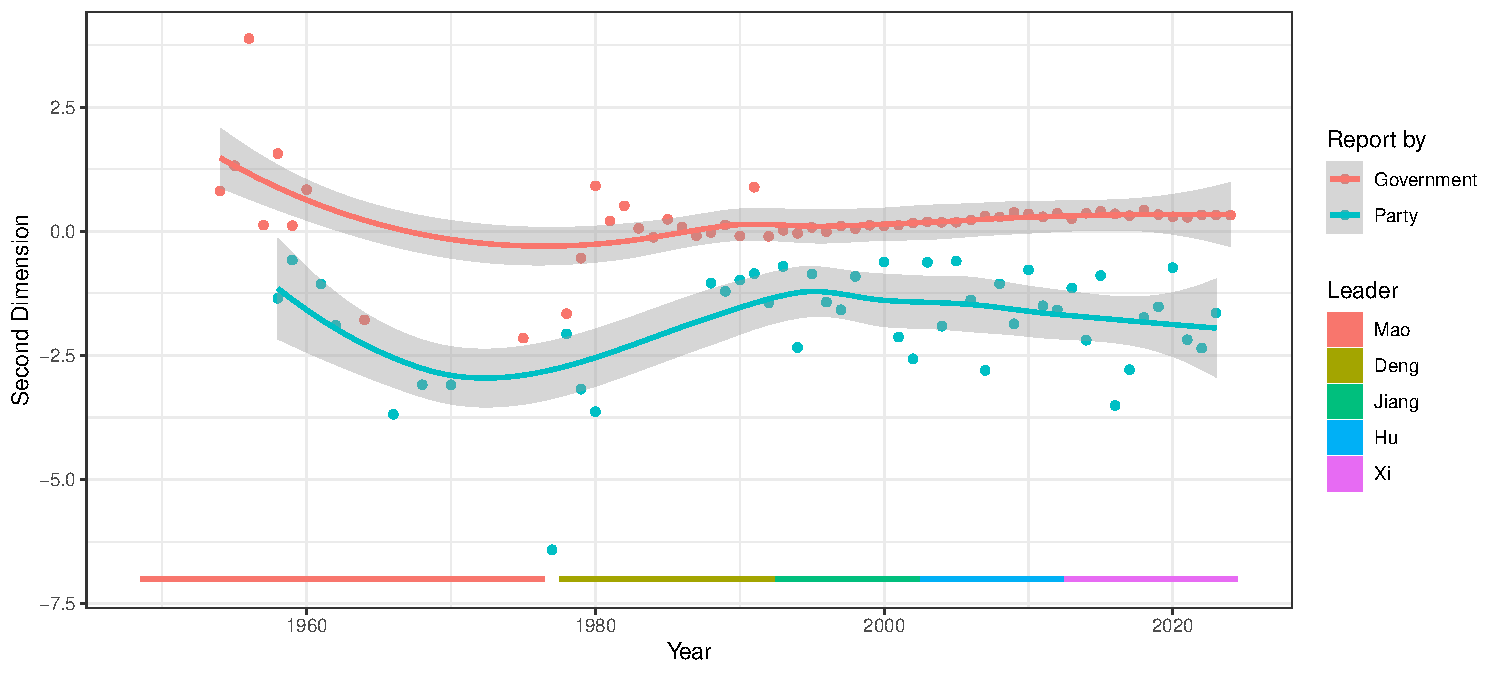
\includegraphics[keepaspectratio]{Maoist_files/figure-pdf/fig-ca-2-1.pdf}}

}

\caption{\label{fig-ca-2}Correspondence analysis of Chinese government
reports and party communiques (second dimension)}

\end{figure}%




\end{document}
